\documentclass[12pt,oneside,onecolumn,openany]{report}      
%\usepackage[nottoc]{tocbibind}
\usepackage[spanish]{babel}
\usepackage[T1]{fontenc} %Paquetes de Fuentes que queramos usar
\usepackage[utf8]{inputenc}
\usepackage{amsmath}
\usepackage{fancyhdr}
\usepackage{graphicx} % Imagenes 
\usepackage{cite} 
\usepackage{multicol}
\usepackage{longtable}
%\usepackage{anyfontsize}
\usepackage{t1enc}
\usepackage[letterpaper, left=3cm, right=2cm, top=2cm, bottom=2cm]{geometry} 
%\usepackage{glossaries}
\usepackage{color}
%\usepackage[export]{adjustbox}
\usepackage{pdfpages}
\usepackage{subcaption}
\usepackage{hyperref}
\usepackage{listings}
\usepackage{float}
\usepackage{enumerate}


\AtBeginDocument{%
  \renewcommand\tablename{Tabla}
  \renewcommand{\bibname}{Referencias}
  \renewcommand{\contentsname}{Índice}
  \renewcommand{\listfigurename}{Índice de Figuras}
  \renewcommand{\listtablename}{Índice de Tablas}

}

% Redefinition of ToC command to get centered heading
\makeatletter
\renewcommand\tableofcontents{%
  \null\hfill\textbf{\Large\contentsname}\hfill\null\par
  \@mkboth{\MakeUppercase\contentsname}{\MakeUppercase\contentsname}%
  \@starttoc{toc}%
}
\makeatother
%Para encabezados y Pies de Pagina
\pagestyle{fancy}
   \lhead{}
    \chead{}
    \rhead{}
    \lfoot{}
    \cfoot{}
    \rfoot{\thepage}


\fancyhead[R]{}
    \renewcommand{\headrulewidth}{0pt}
%   \renewcommand{\footrulewidth}{0.4pt}


\fancypagestyle{plain}{%
    \renewcommand{\headrulewidth}{0pt}%
    \fancyhf{}%
    \fancyfoot[R]{\thepage}%
}

 


%opening
%\title{}
%\author{}

\begin{document}

\begin{titlepage}
	\parbox{2cm}{
	\begin{picture}(18,4)
	    \put(-21,240){
\includegraphics[width=2cm,height=3cm]{./images/IPN.jpg}}
	    \put(0,-280){
\includegraphics[width=0.5cm,height=18.3cm]{./images/lineaAzul.jpg}}
	    \put(-21,-335){
\includegraphics[width=2cm,height=3cm]{./images/ESCOM.jpg}}
	    \end{picture}}
	\parbox{14cm}{\vspace{1cm} 
	    
	    {\fontsize{19}{30} \textbf{  INSTITUTO POLIT\'ECNICO NACIONAL}}
	    \begin{center}
	    {\fontsize{16}{20} \textbf{Escuela Superior de C\'omputo}}\vspace{1cm}\\
	    {\fontsize{18}{20} \textbf{ESCOM}}\vspace{2cm}\\
	    
	    {\fontsize{14}{20} \textit{Trabajo Terminal}}\vspace{1cm}\\
	    {\fontsize{16}{20} \textbf{``Aplicaci\'on de cifrado contra de adversarios clasificadores, para el correo electr\'onico''}}\vspace{1cm}\\
	    {\fontsize{14}{20} \textit{2015-A010}}\vspace{1cm}\\
	    {\fontsize{14}{20} \textit{Presentan}}\\
	    {\fontsize{14}{20} \textbf{Arcos Ayala Jonathan\\Zepeda Ibarra Allan Ulises}}\vspace{2.5cm}\\
	    {\fontsize{14}{20} \textit{Directores}}\\
	    {\fontsize{14}{20} \textbf{Dra. Sandra D\'\i az Santiago \\M. en C. Manuel Alejandro Soto Ramos}}\vspace{4.5cm}\\
	    \end{center}

	    \hfill  \fontsize{14}{20} \textbf{Noviembre 2015}
	    
	}
\end{titlepage}



\tableofcontents
\listoffigures

\listoftables
\newpage

\chapter*{Introducci\'on}
\label{cha:introduccion}
\addcontentsline{toc}{chapter}{Introducción}
Actualmente, una gran cantidad de personas hacen uso del internet y de las nuevas tecnologías para comunicarse. Con ello, también se incrementa la cantidad de información que se transmite y/o almacena. En diversas ocasiones, esta información es susceptible a sufrir distintos tipos de ataques, tales como acceso no autorizado, modificación o destrucción de la misma, entre otros. Adicionalmente, cada día aparecen nuevos tipos de ataques a los sistemas de información. Por lo tanto, surge la necesidad de proteger dicha información.\\
Una de las tecnologías ampliamente usada para comunicarse es el correo electrónico \cite{@}. Los mensajes que envían y reciben los usuarios de correo electrónico pueden ser de diferentes tipos: personales, transaccionales, de notificación o de publicidad. Por lo tanto, cada vez que se escribe y envía un correo electrónico, se está revelando información acerca de las preferencias y/o intereses del usuario. Estos datos, son el insumo más importante, para distintas entidades, entre las cuales están empresas que realizan publicidad en línea, proveedores de internet, instituciones de gobierno, entre otros \cite{sp}.
El propósito de tener estos datos puede ser realizar publicidad efectiva, vender los datos a empresas de publicidad o averiguar si determinado usuario es una amenaza para el gobierno. Para obtener información acerca de los intereses y/o preferencias del usuario, se hace uso de programas de cómputo denominados \textit{clasificadores}. Los clasificadores son herramientas informáticas que analizan una gran cantidad de información, haciendo uso de técnicas de aprendizaje máquina \cite{stanford}, y posteriormente clasifican un mensaje en determinada categoría o perfil. 
En este contexto, los clasificadores pueden constituir una amenaza para algunos usuarios del correo electrónico, por tal motivo de ahora en adelante a los programas que clasifican se les denominará \textit{adversarios clasificadores}.\\
Ante tal escenario, surge la pregunta ¿cómo se puede proteger un usuario contra los adversarios clasificadores?. Una posible respuesta es hacer uso de algoritmos de cifrado estándar. Sin embargo, hacer uso de tales algoritmos, implica que los participantes en la comunicación acuerden una clave de cifrado. Desafortunadamente, acordar una clave, no es un proceso sencillo para el usuario común. Otra desventaja de esta primera solución, es que los algoritmos de cifrado estándar ofrecen un alto nivel de seguridad, el cual resulta excesivo cuando se consideran los recursos y el objetivo de un adversario clasificador \cite{clas}.

\chapter{Marco Teórico} % (fold)
En  este  capítulo  hablaremos  sobre  el  correo  electrónico  y  algunos  de  los intermediarios que hacen posible que este servicio sea usado en toda la red de  internet, también  hablaremos  de  las  amenazas a  las  que  se  tiene  que  enfrentar  este  servicio para  hacer  llegar  información  de  un  usuario  a  otro  de  una  manera  segura  y  cuales  han 
sido   las   respuestas   de   los   proveedores   de   servicio   de   correo   electrónico   para proporcionar dicha seguridad a los usuarios. 
\begin{itemize}

\item \textbf{Correo electrónico} \\
El  correo  electrónico  es  el  servicio  de  internet  por  el cual  se  pueden  enviar  mensajes entre 2 usuarios que cuenten con este servicio. El correo electrónico o “e-mail”
 por sus siglas en inglés, basa su funcionamiento en las oficinas postales. Tomando esa analogía podemos  decir  que  los  usuarios  tienen  cartas  (mensajes  de  correo  electrónico)  que desean  enviar  a  otros  usuarios;  estas  cartas  son  enviadas  a 
las  oficinas  postales (servidores de correo electrónico) donde se almacenan con otras cartas que van dirigidas a otros usuarios en diferentes ciudades; estas oficinas postales envían  las cartas a otras 
oficinas postales  si es  necesario;  y por  último cada oficina postal se  encarga de colocar el mensaje en el  buzón del usuario correspondiente (buzón  de  correos  electrónicos).

\item \textbf{Mensaje de correo electrónico}
Los  mensajes  de  correo  electrónico  al  igual  que  las  cartas  tienen  la  dirección  del receptor, la dirección del emisor y el cuerpo del mensaje, pero a diferencia de las cartas 
los correos electrónicos son enviados por internet y necesitan sus propios formatos. Para  poder  enviar  un  mensaje  de  correo  electrónico  es  necesario  tener  los siguientes  elementos 
como mínimo.\\ 
\textit{Dirección  del  remitente}:\\  Esta  dirección  se  compone  por  dos  elementos  importantes,  el primero es el nombre de usuario seguido de un carácter “@”, el segundo elemento es 
el dominio donde está alojado el servicio de correo electrónico.\\ 
\textit{Direcciones  de  los  receptores}:\\  En  un  correo  electrónico  debe  haber  al  menos  una dirección  de  receptor  para  ser  enviado,  esta  dirección  de  receptor  tiene  la  misma 
estructura que la dirección del remitente.     \\  
\textit{Contenido  del  mensaje}:\\  Es  el  texto  que  se  desea  transmitir entre  el  remitente  y  el receptor. \\ 
El mensaje de correo electrónico cuenta con más elementos pero estos son opcionales y se pueden consultar en el RFC 2821 extensión MIME. 
\item \textbf{Dominio de internet}\\
Es un nombre que identifica a los diferentes dispositivos interconectados en una red sin la  necesidad  de  aprenderse  un  número  de  red.  Estos  dispositivos  pueden  proporcionar 
diferentes servicios como el servicio de correo electrónico. 
\item \textbf{Buzón de correo electrónico}
Un  buzón  de  correo  electrónico  es  un  espacio  virtual  proporcionado  por  el  servicio  de correo electrónico que sirve para almacenar los mensajes enviados y recibidos. 
\item \textbf{Usuario de correo electrónico}
Se  le  conoce  como  usuario  de  correo  electrónico  a  la  persona  que  se  registra  en  un dominio  para  obtener  los  servicios  de  mensajería  proporcionados  por  un  servidor  de correo electrónico. 
\item \textbf{Cliente de correo electrónico}
El  cliente  de  correo  electrónico  es  una  interfaz  por  la  cual  el  usuario  de  correo  electrónico puede administrar sus mensajes enviados y recibidos. \\
El cliente de correo electrónico puede ser de diferentes tipos como son: 

 \textit{Cliente de correo electrónico para la pc}:\\
Estos clientes de correo electrónico son instalados en una computadora y es configurado para sincronizarse con un servidor de correo electrónico cada cierto tiempo o cuando el usuario se lo indique. 
Una  de  las  principales  características  de  éste  cliente  de  correos  es  la  capacidad  de descargar los mensajes del servidor a la computadora para ser leídos sin la necesidad de tener  una  conexión  de  internet  y  en  cuanto  tiene  conexión  con  el  servidor  otra  vez 
descarga los nuevos mensajes y envía los que se tienen pendientes en la computadora. 

 \textit{Cliente de correo electrónico web}:\\
Los  clientes  web  necesitan  un  explorador  de  internet  y  una  conexión  permanente  a  la red  para  que  funcione,  estos  clientes  normalmente  son  proporcionados  por  el  mismo servidor de correo electrónico y nunca descarga los correo en las computadora donde son utilizados. 

 \textit{Cliente de correo electrónico para móviles}:\\
Un  cliente  de  correo electrónico  móvil  se  caracteriza  por  ser una  aplicacion  instalada  en  un dispositivo  móvil. Esta aplicación descarga una copia temporal de los últimos mensajes recibidos.  





\end{itemize}

\section{Servidor de Correo electrónico}
Un servidor de correo electrónico es un programa que se encarga de enviar y recibir los mensajes de correo electrónicos de sus usuarios registrados, este servidor puede recibir 
mensajes  de  usuarios  de  otros  servidores  de  correos  que  sean  dirigidos  a  sus  usuarios registrados. \\
Este  servidor  tiene  que  seguir  algunos  estándares  que  existen  en  internet  para  el  envío(protocolo smtp)  y recepción(protocolo pop3 o imap) de mensajes de correo electrónico. 
\section{Protocolo SMTP}
El protocolo SMTP significa “protocolo para transferencia simple de correo” o “Simple Mail  Transfer  Protocol”   por  sus  siglas  en  inglés,  el  cual  se  encarga  de  enviar  los 
mensajes de correo electrónicos entre dispositivos que se encuentran interconectados en la  red  o  en  internet.  Este  protocolo  solo  se  utiliza  para mandar  los  mensajes  entre 
servidores  o  entre  el  usuario  emisor  y  su  servidor  de  correo  electrónico.  Podemos revisar el protocolo completo en el RFC5321\cite{RFC5321}.
\section{Protocolo POP3}
Este protocolo se encarga de descargar los mensajes del servidor a un cliente de correo electrónico  que  el  usuario  haya  configurado  previamente.  Una  de  las  características  es 
que  solo se sincroniza para  la descarga de  los  mensajes de  correo y  no deja una copia de seguridad en el servidor de correo electrónico. Podemos consultar el funcionamiento detallado en el RFC1939 \cite{1939}.
\section{Protocolo IMAP}
Este  protocolo,  al  igual  que  el  protocolo  POP3,  se  encarga  de  la descarga  de  los mensajes  del  servidor  a  un  cliente  de  correo  electrónico  con  la  diferencia  de  que  la 
sincronización  entre  el  servidor  de y  el  cliente   es continua,  manteniendo  una  copia  de  seguridad  en  el  servidor.  Con  este  protocolo  es 
posible tener varios clientes de correo configurados con la misma  cuenta y los cambios que se realicen en cualquiera de los clientes de correo se verán reflejados en el servidor 
y  en  los  diferentes  clientes  sincronizados.  Este  protocolo  puede  ser  consultado  en  el RFC 6851\cite{6851}.\\ \\
Como hemos podido ver en el presente documento, el servicio de correo electrónico es un  canal  de  comunicación  que  se  ayuda  de  varios  elementos  para  completar  la 
comunicación  entre  dos  usuarios  de  correo  electrónico,  no  importando  que  estos  estén registrados en 2 servidores de correo diferentes. Pero 
para poder entender por completo el  comportamiento  de  este  servicio  tenemos  que  definir  ciertas  características  de  este servicio. 
\\
Este servicio establece una comunicación no orientada a conexión, lo que significa que el  receptor  no  necesita  estar  conectado  al  servicio  de  correo  electrónico  para  recibir  el mensaje en su buzón de correo electrónico. 
\\
Los mensajes enviados por medio del correo electrónico transitan por el   internet   como archivos  en  texto  plano,  esto  quiere  decir  que  cualquiera  que  tenga  una  copia  del 
mensaje puede abrir el correo            electrónico    y    leer    el    mensaje    siguiendo    la estructura del protocolo SMTP. 
\\
Además  de  mandar  mensajes  tiene  la  facultad  de  enviar  archivos  multimedia  en  el mismo mensaje de correo electrónico, esta característica ha sido explotada bastante por empresas   privadas   y   de   gobierno   para   tener   comunicados   a   sus empleados, departamentos, proveedores, socios, etc. 
\\
El  correo  permite  enviar  el  mismo  mensaje  a  más  de  un  usuario  sin  la  necesidad  de hacer un mensaje para cada usuario, esto lo han       utilizado     muchas     empresas     de 
publicidad para hacer publicidad a gran   escala y a muy bajo costo, a este servicio se le llama SPAM. 
\\
Este  medio  de  comunicación  es  bastante  rápido  ya  que  se  estima  que  un  mensaje  de correo  electrónico  tiene  que  llegar  a  su  destino  a  más  tardar  en  5  minutos,  no 
importando la ubicación geográfica del        servidor de correo electrónico. 
\\
Las características mencionadas nos dan a notar que el correo electrónico tiene una baja seguridad al momento de enviar los mensajes, ya que la información que mandamos es 
sumamente fácil de leer por cualquiera que pueda tener una copia del mensaje. Si tomamos en cuenta que un mensaje de tiene que saltar 
por  varios  servidores  antes  de  llegar  a  su  destino,  es  fácil  suponer  que  se puede interceptar una copia del mensaje en el envío de servidor a servidor. 
\\
Por  estos  motivos  los  servidores  de  correo  electrónico  han implementado  diversos candados  de  seguridad  para  blindar  la  transferencia  de  mensajes  entre  servidores.  Una 
de  las  maneras  que  han  encontrado  para  proporcionar  dicha seguridad  ha  sido  a través de la implementación de técnicas criptográficas. 
\\
La criptografía moderna se basa en dos corrientes metodológicas que son la criptografía simétrica  y  la criptografía asimétrica. Estas dos técnicas tienen como propósito ocultar 
el  contenido  de  un  mensaje  con  el  fin  de  que  solo  sea  leído  por  aquellos  que  estén autorizados, a esto se le llama cifrado. 
\section{Cifrado}
Es el procedimiento por el cual  la  información es transformada, esta transformación se realiza por medio de un algoritmo de cifrado junto con una clave para obtener un texto 
ilegible,  el  cual  es  llamado  texto  cifrado.  Para  poder  obtener  el  texto  original  es necesario transformar el texto cifrado por medio de un algoritmo inverso al algoritmo de 
cifrado y la llave con que fue cifrado, esto es llamado algoritmo de descifrado. \\
Como  ya  fue  mencionado  la criptografía simétrica  y asimétrica  llevan a cabo  la  misma tarea  pero  a  través  de  diferentes  esquemas.  Esto  les  proporciona  diferentes  características, tanto en seguridad como en implementación. 
\section{Cifrado Simétrico}
El Cifrado Simétrico es un método criptográfico en el cual se usa una misma clave para cifrar y descifrar mensajes.\\
La clave al  ser usada tanto en el cifrado como en el descifrado se convierte en  la parte más  vulnerable  del  método,  esta  vulnerabilidad  es  contrarrestada  con  el  tamaño  de  la 
clave. El tamaño de la clave es medido por medio del número de bits que la conforma, porque  al  tener  una  clave  con  más  bits  tendremos  un  campo  de  posibles  claves  más 
amplio.  Por  ejemplo,  una  clave  de  56  bits  tiene  256  combinaciones  que  a  su  vez  son 72.057.594.037.927.936  claves  posibles,  este  espacio  de  claves  tan  amplio  dificulta  al 
atacante el obtener fácilmente la clave.\\
Otra de las condiciones que se deben de cumplir para este esquema de cifrado se lleve a cabo  es  el  intercambio  de  claves  entre  los  participantes  de  la  comunicación.  Este intercambio de claves tiene que darse antes del envío de los mensajes.
%\section{Cifrado Asimétrica}
%Este  método  criptográfico  propone  la  generación  de  dos  claves,  de  las  cuales  una  es privada  y  está al resguardo del propietario del par de claves;  la otra clave es pública  y puede ser vista por cualquier usuario que quiera enviarle un mensaje al propietario.
%\\
%Estas  claves  son  mucho  más  grandes  que  las  claves  de  cifrado  simétrico  y  siempre  se generan por pares, haciéndolas claves dependientes una de
 %la otra, esto con el fin de que solo exista una clave privada que descifre lo que cifra su clave pública y viceversa. Este método  de  cifrado  también  cambia  el  esquema  de  envío  de  mensajes  entre  usuario  ya 
%que antes de empezar la comunicación los interlocutores tienen que buscar las claves públicas y una vez que tienen las claves públicas los mensajes son cifrados de la siguiente manera:
%\begin{enumerate}
 %\item El  interlocutor  1  toma  su  mensaje  y  es  cifrado  con  la  clave  pública  del interlocutor 2 obteniendo un texto cifrado. 
 %\item Se envía el texto cifrado al interlocutor 2.
 %\item El interlocutor 2 toma el texto cifrado y lo descifra usando su clave privada para obtener el mensaje del interlocutor 1. 
%\end{enumerate}
%Este método de cifrado propone dar solución a 2 problemas, el primer problema es que para hacer el intercambio de llaves en un cifrado simétrico es muy difícil ya que al pasar 
%la  clave  por  un  canal  inseguro  y  se  intercepta  esta  clave la  comunicación  quedaría expuesta  a  un  ataque.  Este  problema  es  resuelto  con  la  clave  pública  ya  que  esta  llave 
%puede ser  vista por cualquier persona  y tiene  la cualidad de que si  se quiere obtener  la clave privada a partir de la pública sus cálculos son demasiado difíciles de resolver.
%\\
%El  segundo  problema  es  el  manejo  de  claves  para  establecer  comunicaciones  seguras con  más  de  un  usuario.  Tomando  el  modelo  de  cifrado  simétrico  necesitaríamos  tener 
%una clave diferente para cada conexión segura que se desea establecer, mientras que en el  cifrado  asimétrico  se  necesita  tener  un  par  de  claves, 
%pública  y  privada,  por  cada usuario y esas claves son suficientes para hacer las conexiones seguras que se requieran. 
%\\
%El  beneficio  que  se  tiene  al  utilizar  claves  públicas  se  ve  al  momento  de  establecer comunicaciones  seguras,  por  ejemplo  si  tuviéramos  6  usuarios  en  una  red  con  un 
%esquema  de  cifrado  asimétrico  solo  se  necesitaría  publicar las  claves  públicas  de  los usuarios  en  un  lugar  común  para  los  6,  y  cada  vez  que  se  quiera  establecer  una 
%comunicación segura con algún usuario solo tienen que buscar su clave pública y cifrar el mensaje sin la necesidad de ponerse de acuerdo con cada 
%uno de los usuarios de la red para  establecer  una  clave  para  cada  comunicación  que  se  desea  establecer  como  en  el cifrado simétrico.
%\\ \\
A  pesar  de  la  implementación  de  estas  técnicas  criptográficas  los  ataques  a  las comunicaciones  siguen  existiendo  y  estos  ataques  se  han  clasificado  dependiendo  de 
cuanta  información  tenga  disponible  el  adversario  para  poder  romper  el  cifrado  y obtener la información deseada. 

Nosotros  nos  enfocaremos  a  un  tipo  de  ataque  llamado “ataque  de  texto  cifrado” o COA  que  hace  referencia  a  su  nombre  en  inglés “
Ciphertext-only  attack”\cite{Ciphertextonly}.  Este ataque  solo  cuenta  con  los  textos  cifrados  que  va  recopilando  de  un  canal  o  base  de 
datos,  estos  textos  cifrados  los  utiliza  para  hacer  un  análisis  criptográfico  de  cómo  se comporta la técnica de cifrado  y trata de hallar el texto en claro a partir de los textos cifrados que va recopilando. 
\\
Este  tipo  de  ataques  es  muy  común  en  el  internet  aunque  con  muy  baja  efectividad cuando   se   implementa   en   comunicaciones   altamente   protegidas,   y   cuando   se 
implementa en canales de comunicación desprotegidos  la  información obtenida  llega  a ser  muy  pobre.  En  los  últimos  años  se  han  dado  cuenta  que  si   este  tipo  de 
agentes   atacan las  comunicaciones  sin  cifrado se  obtienes  características  valiosas  sobre  los usuarios  que  utilizan  este  tipo  de  canales  de  comunicación,  este  tipo  de  ataques  son 
ejecutados por programas llamados agentes clasificadores.

El método de cifrado asimétrico se ha implementado en diversos esquemas para proporcionar seguridad en las comunicaciones de internet, pero en la actualidad algunas de ellas son tan populares y efectivas que se han utilizado como estándares dentro de la transferencia de información dentro de internet.\\
\section{PGP (Pretty Good Privacy).}
Es un programa desarrollado por Phil Zimmermann y cuya finalidad es proteger la información distribuida a través de Internet mediante el uso de criptografía de clave pública, así como facilitar la autenticación de documentos gracias a firmas digitales.\\
PGP es un sistema híbrido que combina técnicas de criptografía simétrica y criptografía asimétrica, la velocidad de cifrado del método simétrico y la distribución de la claves del método asimétrico.\\
Cuando un usuario emplea PGP para cifrar un texto en claro, dicho texto es comprimido. La compresión de los datos ahorra espacio en disco, tiempos de transmisión; después de comprimir el texto, PGP crea una clave de sesión secreta que solo se empleará una vez. Esta clave es un número aleatorio generado a partir de los movimientos del ratón y las teclas que se pulsen; Esta clave de sesión se usa con un algoritmo para cifrar el texto claro; una vez que los datos se encuentran cifrados, la clave de sesión se cifra con la clave pública del receptor y se adjunta al texto cifrado enviándose al receptor.\\
El descifrado sigue el proceso inverso. El receptor usa su clave privada para recuperar la clave de sesión, simétrica, que PGP luego usa para descifrar los datos.\cite{pgp}\\

\section{Adversarios Clasificadores}
Los agentes clasificadores son programas que se dedican a observar los mensajes que se intercambian  entre  los  usuarios  de  correo  electrónico,  con  el  fin  de  clasificarlos  e 
identificar  a  todos  los  usuarios  que  cumplan  con  cierto  criterio.  Esta  clasificación  se hace de manera masiva y la realiza haciendo una búsqueda de palabras clave dentro de 
los  mensajes de  los usuarios. Por ejemplo, el  clasificador puede estar interesado en  los mensajes  que  contienen  la  palabra  clave  "Bomba",  así  que 
todos  los  mensajes  que contengan esta palabra serán etiquetados en una clasificación en específico, este proceso se lleva a cabo por medio de técnicas de 
“Reconocimiento de patrones” y “Aprendizaje Máquina” para encontrar y clasificar los mensajes que intercepta.\cite{Attacks}\cite{clas}
\\
La  clasificación  de  estos  mensajes  tiene  diversos  usos, ya  que  pueden  ser  clasificados con  fines demográficos, con  fines comerciales o con  fines gubernamentales. Todo esto 
con  el  propósito  de  generar  las  estadísticas  de  comportamientos  e  intereses  de  los usuarios de correo electrónico. 


Después de conocer el funcionamiento de los agentes, podríamos deducir que la solución más simple y obvia es cifrar el correo haciendo que este
 sea ilegible y siendo que, el agente  clasifica  los  correos  electrónicos  semánticamente  dependiendo  de  las  palabras 
que  encuentra  en  el  correo.
\\

\chapter{Antecedentes} % (fold)
La  única  referencia  que se tiene  sobre  un  esquema  criptográfico  contra  adversarios clasificadores es el que encontramos en el artículo 
“Defending Email Communication Against Profiling” de Philippe Golle  y  Ayman  Farahat, ambos  miembros del 
“Palo Alto Research Center”.\\
En su artículo se aborda el ataque de adversarios clasificadores sobre los mensajes de correo electrónico. En este articulo proponen un protocolo para la comunicación por correo electrónico, el cual funciona con una función  de cifrado que sustituye cada una de las palabras del mensaje por otra de la misma extencion y frecuencia gramatical (esta función esta pensada para texto en idioma ingles). Esta función tiene como parámetro una clave K. Para calcular esta clave se usan los datos de cabecera que acompañan el mensaje (dirección  del remitente, la dirección del destinatario, la hora a la que se envía el correo electrónico y potencialmente otros campos), estos datos se introducen en una función hash lenta (que puede ser una función hash conocida, con una complejidad de calculo moderadamente mas alta) el resultado de esta función es la clave K. \\
Este  protocolo resulta inseguro para la criptografia clásica pero es efectivo contra el ataque de clasificadores. Por otro lado este protocolo resuelve dos problemas, le  permite  a los usuarios  calcular  la  clave de cifrado y descifrado  fácilmente  ya  que  estos los datos con que se calcula son  públicos, resolviendo así el intercambio de claves. Al usar un cifrado de tipo semántico permite que el texto se vea como una texto en ingles pero indistinguible para los clasificadores. 
\\
Tomando  en  cuenta  que  esta  es  la  única  referencia  sobre el  tema  que  estamos abordando, podemos decir que trabajamos en el mismo sentido ya que esta propuesta de 
solución está  basada en el  artículo “On Securing  Communication  from Profilers”\cite{clas,Attacks} en el que  se  propone  algo  similar  en  cuanto  al  cifrado,  nos  lleva  a  tomar  muy  en  cuenta  el 
poder del algoritmo de cifrado que se usará en nuestra propuesta de solución.

\chapter{Objetivos} % (fold)
\label{cha:objetivo}
\addcontentsline{toc}{chapter}{Objetivos}

    \section{Objetivos Generales} % (fold)
    \addcontentsline{toc}{section}{Objetivos Generales}
    \label{sec:objetivos_generales}
      Desarrollar  una  herramienta  para  un  cliente  de  correo  electrónico  que  permita  cifrar  el 
      contenido  de  los  mensajes  para  evitar  su  clasificación, haciendo uso de tecnicas criptograficas simetricas y un servidor que verifique el envio y recepción de CAPTCHAS entre usuarios. 
    \section{Objetivos Específicos} % (fold)
    \addcontentsline{toc}{section}{Objetivos Específicos}
    \label{sec:objetivos_especificos}
        \begin{enumerate}
         \item Desarrollar  una  herramienta  en  un  cliente  de  correo  electrónico  para  el  envío  y recepción  de   los   correos  cifrados   y   la  generación,  envío  y  recepción  de CAPTCHAS. 
         \item Desarrollar un servidor de llaves que reciba, aloje y envíe los CAPTCHAS a los usuarios para descifrar los correos electrónicos.       
         \item Desarrollar un algoritmo de cifrado y descifrado basado en el envío y recepción de CAPTCHAS.
        \end{enumerate}
        
\chapter{Justificación}
Lo que se pretende en este trabajo terminal, es ofrecer al usuario una solución alternativa para proteger al correo electrónico, contra los clasificadores. Dicha solución se considera más fácil de usar y además ofrece un nivel de seguridad adecuado, teniendo en cuenta las características de los clasificadores. La solución que se propone, hará uso de CAPTCHAs y de un algoritmo criptográfico. Los CAPTCHAs son programas de cómputo, cuyo propósito es distinguir si están interactuando con una máquina o con un ser humano. 
Este algoritmo criptográfico tiene una gran ventaja al momento de la generación de llaves, ya que sus llaves son simétricas a diferencia de muchos algoritmos estándares que utilizan una generación de un par de llaves asimétricas, estos algoritmos criptográficos asimétricos nos llevan a necesitar una comunicación previa entre el emisor y el receptor del mensaje enviado. Mientras que al usar el esquema aquí propuesto solo es necesario que el emisor genere una llave, la transforme y envíe los CAPTCHAs, y que el receptor resuelva los CAPTCHAs, recupere la llave y posteriormente el mensaje de correo electrónico.
El envío de los correos se propone hacerlo enviando el correo electrónico con el contenido cifrado a un servidor de correo electrónico donde se alojará hasta que el cliente de correos electrónico instalado en el equipo de cómputo del receptor lo descargue por medio del protocolo POP3, al mismo tiempo se enviarán los CAPTCHAs que permiten recuperar la llave de cifrado a un tercer agente llamado servidor de llaves, el cuál verificara que la petición hecha por el receptor es válida y que el receptor es un usuario valido. El protocolo SSL se usará para garantizar el envío de los CAPTCHAs por parte del emisor, la correcta recepción por parte el servidor de llaves y la recuperación por parte del receptor para la correcta recuperación de la llave de cifrado y posterior descifrado de los correos electrónicos. El servidor de llaves es fundamental para el funcionamiento de este sistema, ya que esto le da un nivel de seguridad un poco más elevado que si lo enviáramos todo en un sólo paquete.
        
\chapter{Propuesta de solución}
\clearpage
Tomando en cuenta la información ya vertida en este documento, a continuación se explicará detalladamente la propuesta de solución que hemos ideado.\\
En la figura \ref{fig:4-1-1} tenemos el diagrama general del sistema, se puede apreciar la comunicación entre las diferentes entidades que usaremos, que datos se mandan y reciben y por que canales transitan estos datos. A continuación describiremos de manera general como es el proceso de envío y recepción de correos electrónicos ideado para este esquema.\\
\begin{enumerate}
 \item {Envío}
\begin{itemize}
\item El remitente escribe el correo electrónico y le da enviar.\\
\item El correo electrónico pasa por el complemento del cliente de correo.\\
\item El cliente genera a partir del correo una clave que usaremos para cifrar el mensaje.\\
\item Se cifra y se empaqueta el mensaje con el protocolo SMTP.\\
\item Se coloca una bandera en el mensaje.\\
\item La clave se convierte en CAPTCHA y es enviada al servidor de CAPTCHAS.\\
\item Se envía el mensaje de correo electrónico al destinatario.\\
\end{itemize}

\item{Recepción}
\begin{itemize}
\item El receptor abre un correo electrónico cifrado con el presente esquema.\\
\item El cliente lo descarga del servidor por medio del protocolo POP3 o IMAP.\\
\item Se hace una petición al servidor de CAPTCHAS para recuperar los CAPTCHAS del correo.\\
\item El usuario resuelve el CAPYCHA y se recalcula la clave de descifrado.\\
\item Se descifra el mensaje y se le muestra al usuario.\\
\end{itemize}
\end{enumerate}
\begin{figure}[h]
	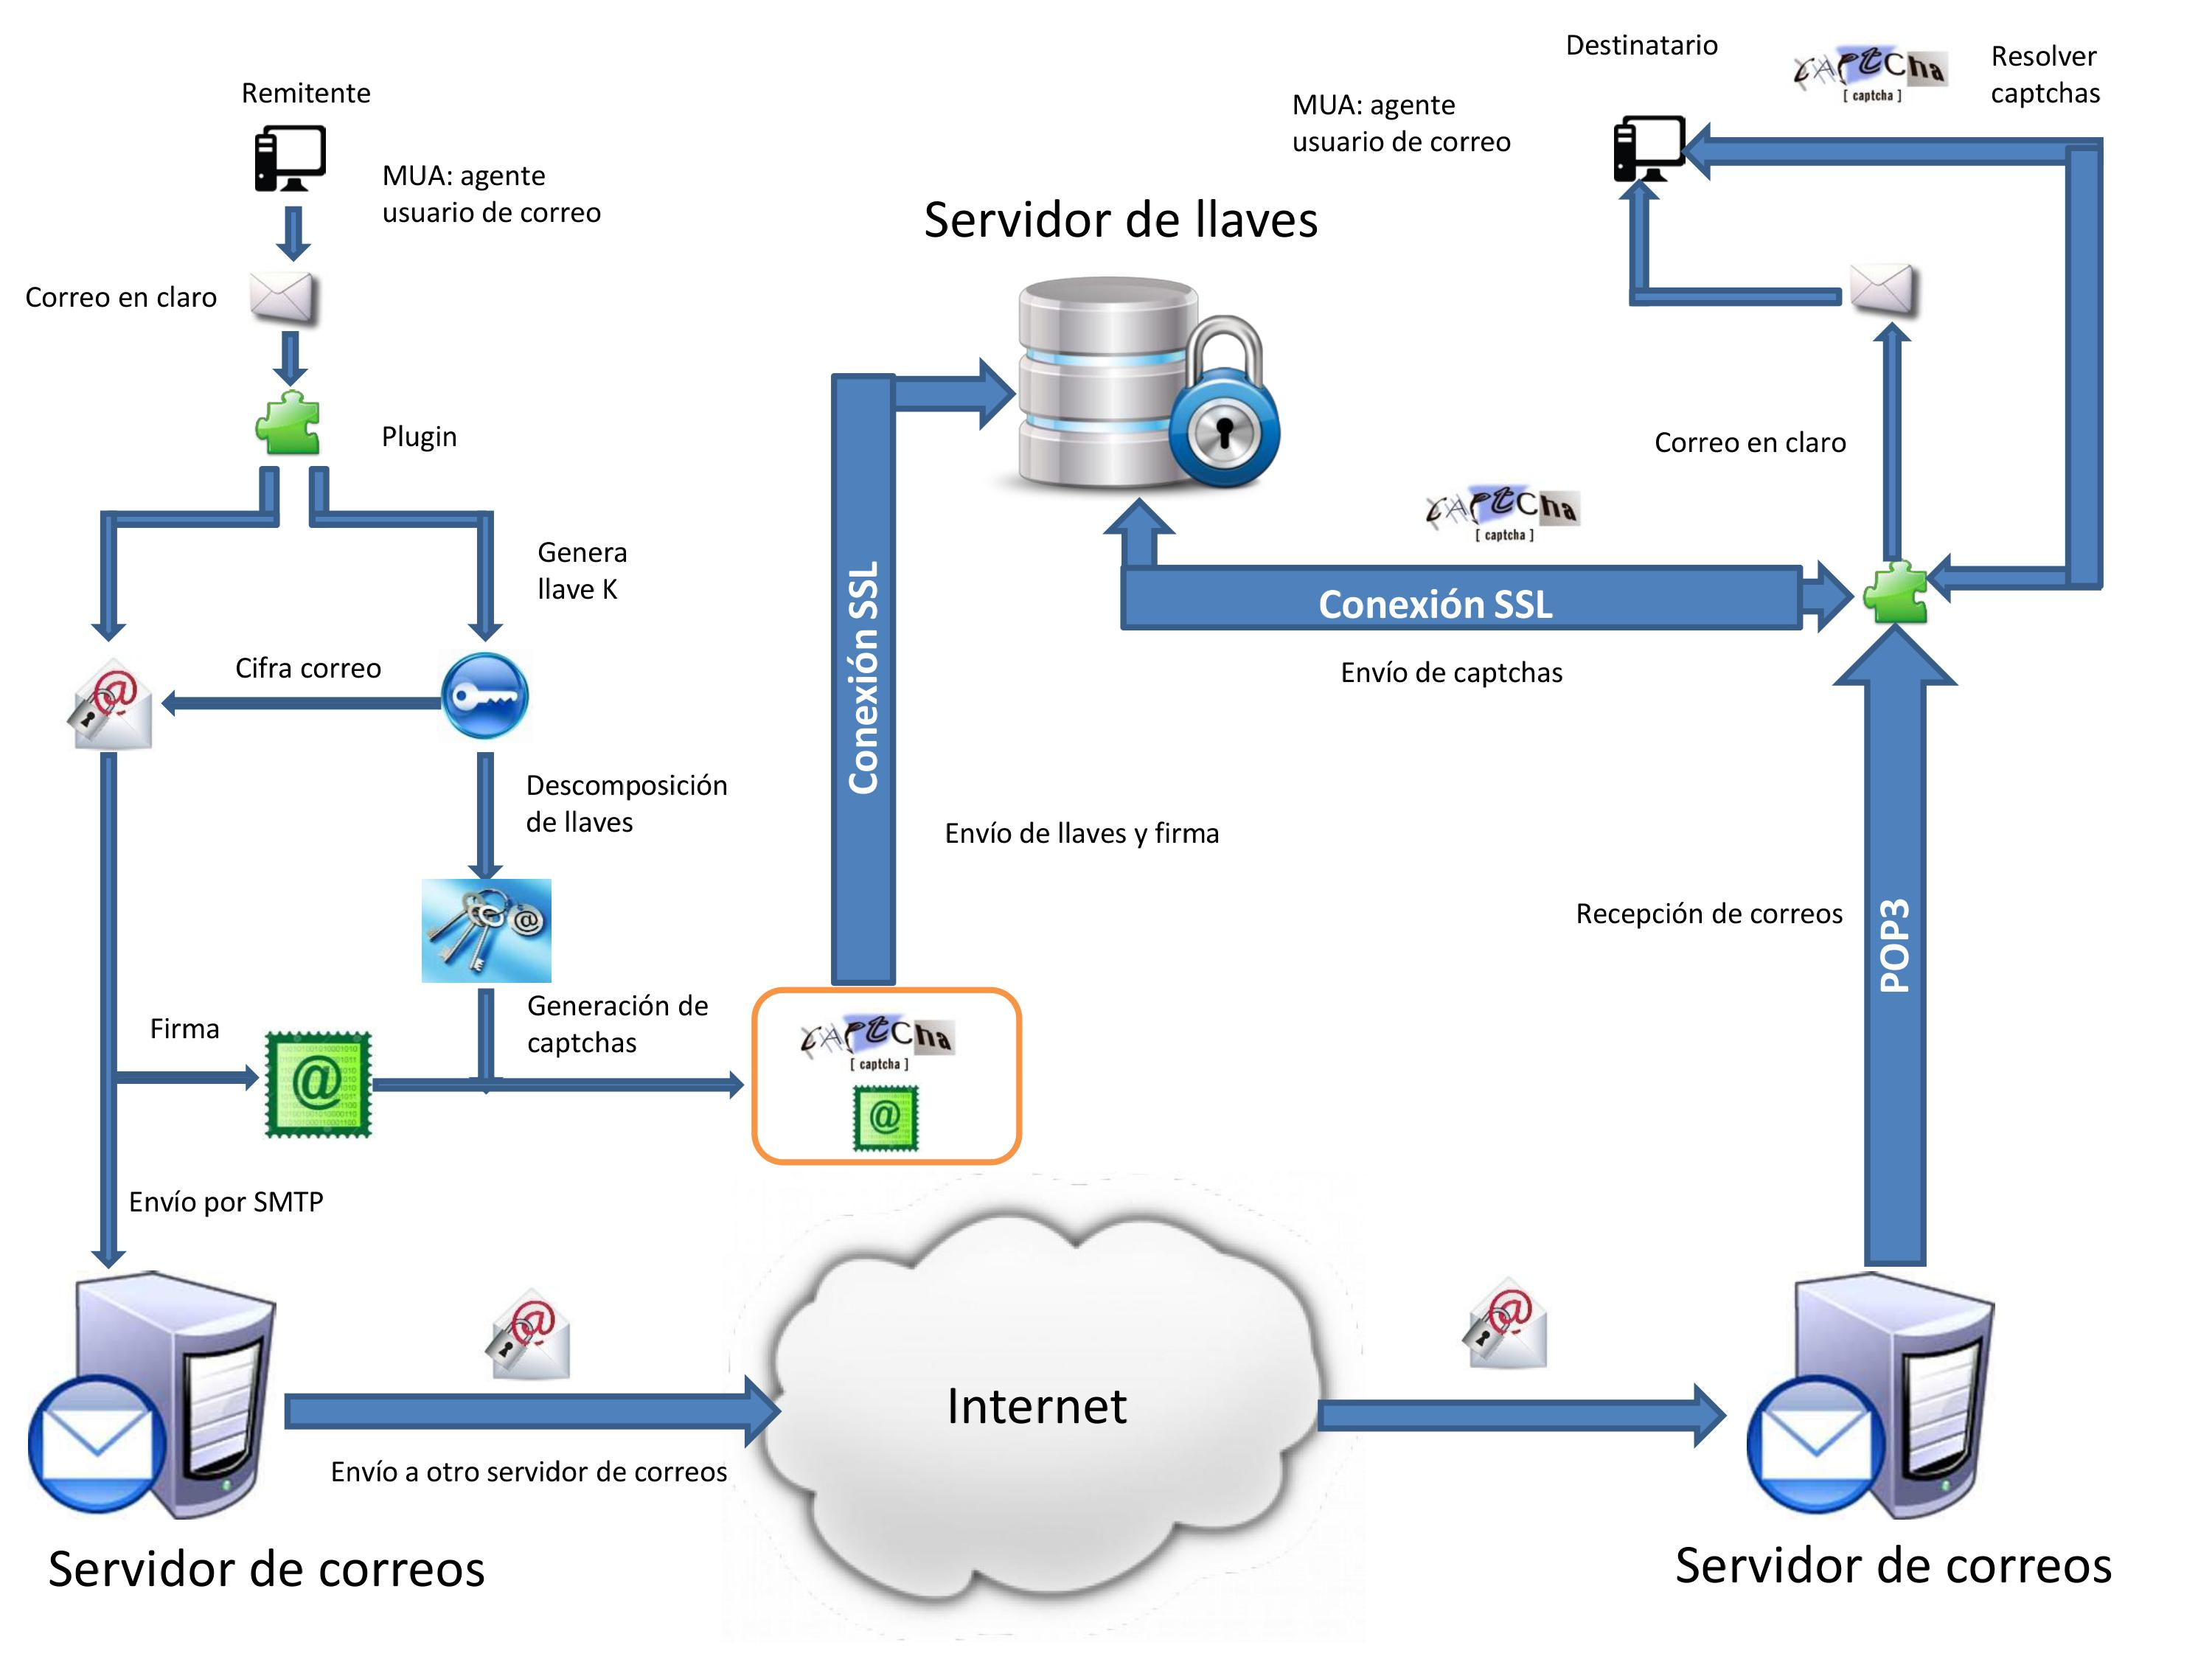
\includegraphics[width=1\linewidth, height=10cm]{./images/0001.jpg}
	\caption{Diagrama General del sistema}
	\label{fig:4-1-1}
\end{figure}
\section{Tecnologías}
Como ya hemos visto en el esquema anterior necesitamos hacer uso de las herramientas adecuadas para poder desarrollar este esquema de cifrado. Las herramientas que analizaremos se describen en las siguientes secciones.\\
\subsection{Cliente de correo electrónico}
Un cliente de correo electrónico es necesario para el desarrollo de este proyecto ya que en él se instalará un complemento que cifre el mensaje, envie los CAPTCHAS y descifre los mensajes de correo electrónico. Para ello buscamos un cliente de correo electrónico que cuente con el soporte de los protocolos POP3, SMTP y IMAP; sus licencias son de código libre; soporte la instalación de APIs externas; y tenga soporte en los sistemas operativos \textbf{\textit{Windows}}, \textbf{\textit{IOS}} y \textbf{\textit{Linux}}. Por lo tanto se investigaron los siguientes clientes de correo electrónico que se encuentra en el mercado: \\
\begin{longtable}[H]{| p{2,5cm} | p{2cm} |p{2cm}|p{1,5cm}|p{2cm}|p{3cm}|p{2cm}|}%\footnotesize
 \hline
 \textbf{Cliente de correo electrónico}&\textbf{Sistema Operativo}&\textbf{Protocolos soportados}&\textbf{Código Libre}&\textbf{Agregar funcionalidad}&\textbf{Extra}&\textbf{Gratuita o de paga}\\
 \hline
 \textbf{eM client}&Windows 7, 8 \& 10 ; IOS&POP3, SMTP, IMAP, EWS, AirSyn&NO&NO&100\% compatible con gmail y sus APIs&Ambos\\
 \hline
 \textbf{Postbox}&Windows, IOS&POP3, SMTP, IMAP&NO&SI por medio de APIs&Sincronización con Dropbox, OneDrive, Facebook y Twitter&Ambos\\
 \hline
 \textbf{Zimbra}&Windows, IOS \& Linux&POP3, SMTP, IMAP&SI&SI por medio de APIs&Una plataforma de nivel empresarial y capas se soportar sincronización con múltiples servicios&Ambos\\
 \hline
 \textbf{Opera Mail}&Windows, IOS \& Linux&POP3, SMTP, IMAP&SI&NO&La plataforma para desarrollar en Opera se actualiza cada semana&Gratuito\\
 \hline
 \textbf{Thunderbird}&Windows, IOS \& Linux&POP3, SMTP, IMAP&SI&SI por medio de APIs&Cliente de correo versátil y fácilmente escalable y una comunicad de desarrollo bastante amplia&Gratuito\\
\end{longtable}
\begin{itemize}
 \item El cliente de correo electrónico \textbf{\textit{eM client}} tiene una sincronización a 100\% con las cuentas de \textbf{\textit{Gmail}} y sus APIs, cuenta con una versión gratuita y una versión de paga; puede hacer migración de mensajes de correo electrónico y contactos de diversos clientes de correo electrónico y tiene una compatibilidad con muchos servidores de correo electrónico.\cite{em}\\Su desventaja es que su código es cerrado y permite agregar funcionalidades.
 \item El cliente de correo electrónico \textbf{\textit{Postbox}} esta soportada en los sistemas operativos \textbf{\textit{Windows 7}} o posteriores y \textbf{\textit{IOS}}, esta aplicación es generada por el servidor de correo electrónico \textbf{\textit{Postbox}} por lo tanto cuenta con una sincronización al 100\% con este servidor, también soporta otros servidores de correo como \textbf{\textit{Gmail}} y \textbf{\textit{Outlook}}; este cliente puede sincronizarse con \textbf{\textit{Dropbox}}, \textbf{\textit{Onedrive}} y redes sociales como \textbf{\textit{Facebook}}, \textbf{\textit{Twitter}}, entre otras. Es posible agregar más funcionalidades con la instalación de APIs.\\Una desventaja de esta aplicación es que su código es cerrado, pero gracias a que esta basado en código de \textbf{\textit{Mozilla}} puedes desarrollar APIs para agregarle tus propias funciones. \cite{box}
 \item El cliente de correo electrónico \textbf{\textit{zimbra}} es la aplicación más completa que se analizó, tiene compatibilidad con el servidor \textbf{\textit{zimbra}} pero es capaz de soportar otros servidores de correo electrónico, se encuentra en los 3 sistemas para PC, \textbf{\textit{Windows}}, \textbf{\textit{IOS}} \& \textbf{\textit{Linux}}, da la facilidad de agregarle funcionalidades por medio de la instalación de APIs y gracias a que su código es abierto se pueden programar funciones propias. Este cliente cuenta con la versión gratuita y la versión de paga. Una gran ventaja que tiene es que puedes certificarte en el desarrollo APIs para este cliente de correo electrónico.\cite{zim}\\La única desventaja que encontramos en este cliente de correo es que la plataforma es demasiado grande y el tiempo que se necesita invertir al estudio del código es demasiado y el tiempo de desarrollo de este proyecto es muy corto.
 \item \textbf{\textit{Opera mail}} es un cliente de correo electrónico que salió al mercado recientemente y se puede instalar en los sistemas operativos \textbf{\textit{Windows}}, \textbf{\textit{IOS}} \& \textbf{\textit{Linux}}, es capaz de comunicarse con diversos servidores de correo electrónico y su código es de libre acceso.\\Su principal desventaja es que las funcionalidades que se quieran agregar no pueden ser adquiridas por medio de la instalación de complementos o APIs.\cite{opera}
 \item Por último tenemos a \textbf{\textit{Thunderbird}} que es un cliente de correo electrónico desarrollado por \textbf{\textit{Mozilla}}, este cliente es de código abierto y la instalación de APIs para agregar funcionalidad es demasiado sencilla; es un cliente de correo que puede ser instalado en los sistemas operativos \textbf{\textit{Windows}}, \textbf{\textit{IOS}} y \textbf{\textit{Linux}}.\cite{thun}
\end{itemize}
Por lo tanto el cliente de correo electrónico que utilizaremos será \textbf{\textit{Thunderbird}} al ser un cliente de correo electrónico casi tan completo como \textbf{\textit{zimbra}} pero con la facilidad de desarrollar APIs más rápido.\\
\subsection{Lenguajes de programación.}
Uno de los objetivos que se tienen en este proyecto es generar un complemento para un cliente de correo electrónico por lo tanto al escoger a \textbf{\textit{Thunderbird}} como cliente tenemos que programar con el lenguaje que fue desarrollado para tener la mayor compatibilidad.\\Para el desarrollo de este proyecto utilizaremos\cite{thun}:
\begin{itemize}
 \item Lenguaje Python
 \item HTML 5
 \item CSS3
\end{itemize}
A pesar de ser una aplicación de escritorio este cliente de correo electrónico está construido con lenguajes web.
\subsection{Tipos de CAPTCHAS}
En nuestro esquema de cifrado es necesario esconder la palabra que genera clave en un CAPTCHA para ser enviado a otro usuario y descifre el mensaje, pero existen varios tipos de CAPTCHAS que podemos utilizar\cite{cit}.\\Los CAPTCHAS se pueden clasificar de la siguiente forma:
\begin{itemize}
 \item CAPTCHAS de texto: Este tipo de CAPTCHAS genera una pregunta sencilla donde la respuesta a la pregunta es la respuesta al CAPTCHA.
 \item CAPTCHAS de imágenes: Este tipo de CAPTCHAS nos muestran en una imagen una cadena de caracteres distorsionados, esta cadena de caracteres es la repuesta del CAPCHA transformada en una imagen.
 \item CAPTCHAS de audio: Este tipo de CAPTCHAS se caracterizan por  ser un audio con ruidos de fondo, donde nos dirán la respuesta oculta.
 \item CAPTCHAS de video: Este tipo de CAPTCHAS nos muestran un video de unos cuantos segundos donde una palabra aparece alrededor de la pantalla, esta palabra es la respuesta al CAPTCHA.
 \item CAPTCHAS de acertijos: Este tipo de CPATCHAS es versatil, ya que se trata de pequeños acertijos que resolver donde la respuesta no es una palabra si no una acción o serie de acciones. Los CAPTCHAS de acertijos pueden ser armar un rompecabezas pequeño, seleccionar la imagen que no corresponde, unir figurar geométricas, etc. 
\end{itemize}
Para poder decidir qué tipo de CAPTCHAS se utilizará se consideró los siguientes puntos:
\begin{itemize}
 \item Facilidad de creación.
 \item Peso en byte del CAPTCHA.
 \item Forma del despliegue.
 \item Tipo de respuesta.
\end{itemize}
Por lo tanto nosotros necesitamos un tipo de CAPTCHA con poco peso, que su respuesta sea una cadena de caracteres y su forma de despliegue sea fácil de implementar. \\
Consideradas las necesidades anteriores las opciones son CAPTCHAS de imágenes y CAPTCHAS de texto, pero en este proyecto utilizaremos los CAPTCHAS de imágenes porque se almacenaras en los CAPTCHAS las claves de cifrado de los mensajes de correo electrónico y estas son cadenas de caracteres que no se les puede generar una pregunta coherente. \\
\subsection{Bases de datos para almacenar los CAPTCHAS.}
Para escoger un gestor de base de datos que controle la información delos usuarios registrados en nuestra aplicación, la información de los  mensajes que envían entre usuarios y los CAPTCHAS asociados a los mensajes para ser descifrados consideramos 3 características principales en un gestor base de datos relacional:\\
\begin{itemize}
 \item Rapidez en transferencias de información.
 \item Número de usuarios conectados que soporta.
 \item Facilidad de comunicación entre los lenguajes Python, HTML con los gestores de base de datos.
\end{itemize}
Los 3 gestores que se analizaron fueron SQLite, MySQL y PostGreSQL.\\
SQLite es un gestor de base de datos sumamente ligero que soporta hasta 2 terabytes de información, esta base de datos es compatible con python y lenguajes de programación web. Este gestor por su misma ligereza es posible ser implementada en dispositivos móviles, pero no es recomendable cuando múltiples usuarios están haciendo peticiones al mismo tiempo ya que su rendimiento baja\cite{DB}.\\
MySQL es un gestor de base de datos que se caracteriza por su transferencia al hacer consultas de datos almacenados; es uno de los gestores libres más utilizados en aplicaciones web y cuenta con diferentes APIs para hacer la comunicación con los lenguajes Python, PHP, C++, etc. Y soporta peticiones de múltiples usuarios gracias a la implementación de hilos.\\
PostGreSQL es un gestor de base de datos que puede hacer operaciones complejas como subconsultas, transacciones y rollbacks’s. Soporta las peticiones de múltiples usuarios pero en cuanto a la velocidad de transferencia de información, comparado con MySQL, es muy lenta pero lo compensa manteniendo una velocidad casi invariable a pesar de que la base se mantenga con un número grande de registros.\cite{sql}\\
Se eligio el gestor de base de datos MySQL porque el proyecto necesita mayor rapidez en la transferencia de información más que generar filtros muy complejos para la búsqueda de información.\\
\clearpage
\chapter{An\'alisis y Dise\~no} % (fold)
\section{Diagramas de caso de uso}
Para el desarrollo de esta propuesta se muestran los siguientes diagramas, estos muestran el diseño que nos da una idea mas clara de como quedara el sistema.
\begin{figure}[H]
	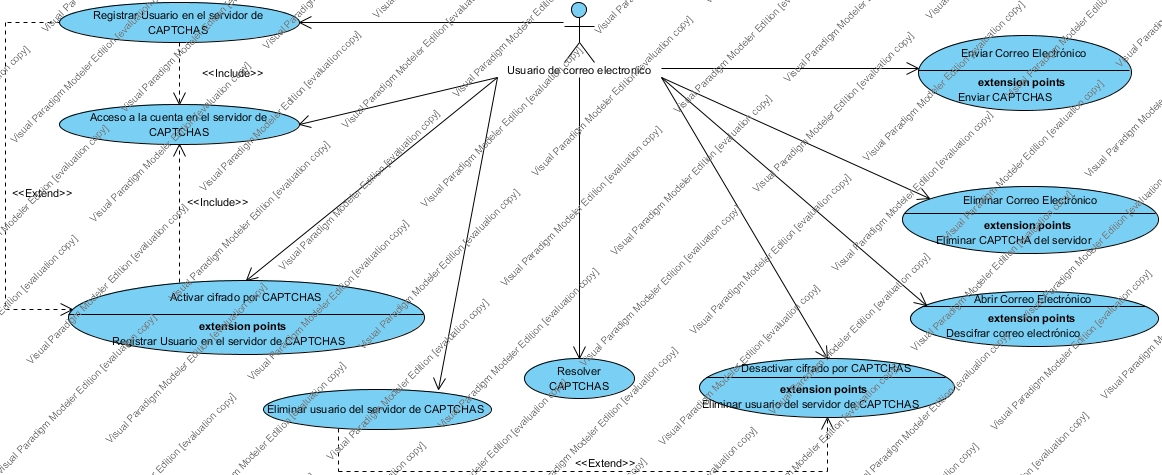
\includegraphics[width=1\linewidth, height=10cm]{./images/casodeuso1.jpg}
	\caption{Diagrama General de caso de uso}
	\label{fig:4-2-1}
\end{figure}
\subsection{Diagrama de caos de uso CU2 Registrar usuario en el servidor de CAPTCHAS}
\begin{figure}[H]
	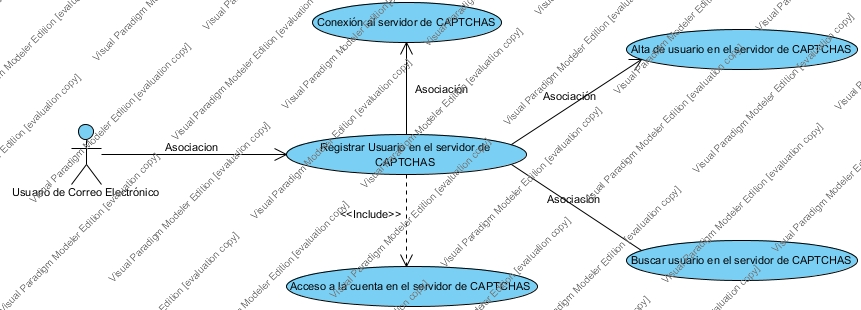
\includegraphics[width=1\linewidth, height=10cm]{./images/casodeuso2.jpg}
	\caption{Diagrama de caos de uso CU2 Registrar usuario en el servidor de CAPTCHAS}
	\label{fig:4-3-1}
\end{figure}

 \begin{longtable}[H]{| p{4,5cm} | p{0,5cm} |p{4cm}|p{5cm}|}%\footnotesize
   %\centering
   %{
     %\begin{tabular}
     \hline
     \textbf{Caso de Uso} &\multicolumn{3}{|l|}{CU2 Registrar Usuario en el servidor de CAPTCHAS}\\
     \hline
     \textbf{Actor} & \multicolumn{3}{|l|}{Actor1. Usuario de Correo Electrónico}\\
     \hline
     \textbf{Descripción} & \multicolumn{3}{|p{10cm}|}{Describe los pasos necesarios para registrar un nuevo usuario en el servidor de CAPTCHAS.}\\
     \hline
     \textbf{Pre-condiciones} & \multicolumn{3}{|l|}{Tener una cuenta de correo electrónico.}\\
     \hline
     \textbf{Post-condiciones} & \multicolumn{3}{|l|}{Activación del módulo de cifrado por CAPTCHAS.}\\
     \hline
     \textbf{Puntos de inclusión} & \multicolumn{3}{|l|}{Acceso a la cuenta en el servidor de CAPTCHAS.}\\
     \hline
     \textbf{Puntos de extensión} & \multicolumn{3}{|l|}{}\\
     \hline
     \textbf{Flujo principal} & & Actor/Sistema & Acción a realizar\\
     \hline
     & 1 & Actor & El usuario selecciona la opción registrarse en el servidor de CAPTCHAS\\
     \hline
     & 2 & Sistema & El cliente de correo contesta un formulario con la información necesaria para dar de alta en el servidor de CAPTCHAS.\\
     \hline
     & 3 & Actor & Completa el formulario y oprime el botón de registrar.\\
     \hline
     & 4 & Sistema & El sistema valida los datos proporcionados por el usuario.\\
     \hline
     & 5 & Sistema & Se conecta con el servidor y valida si el usuario ya está registrado. <FA01 - Usuario ya registrado> <FA02 - Falla en la conexión con el servidor>\\
     \hline
     & 6 & Sistema & Manda la información del usuario y lo da de alta.\\
     \hline
     & 7 & Sistema & Despliega el siguiente mensaje "El usuario se ha dado de alta correctamente"\\
     \hline
     & & & \textbf{Fin del flujo principal}.\\
     \hline
     & \multicolumn{3}{|l|}{\textbf{FA01 - Usuario ya registrado}.}\\
     \hline
     \textbf{Flujo alternativo} & & Actor/Sistema & Acción a realizar\\
     \hline
     & 1 & Sistema & Despliega el siguiente mensaje "El usuario ya está registrado favor de proporcionar otra cuenta de correo electrónico"\\
     \hline
     & 2 & & El flujo continúa en el paso 3 del flujo principal.\\
     \hline
     &  & & \textbf{Fin del flujo alternativo}\\
     \hline
     
     \hline
     & \multicolumn{3}{|l|}{\textbf{FA02 - Falla en la conexión con el servidor}.}\\
     \hline
     \textbf{Flujo alternativo} & & Actor/Sistema & Acción a realizar\\
     \hline
     & 1 & Sistema & Despliega el siguiente mensaje " La conexión con la red es nula o limitada, favor de realizar esta operación más tarde"\\
     \hline
     & 2 & & El flujo continúa en el paso 1 del flujo principal.\\
     \hline
     &  & & \textbf{Fin del flujo alternativo}\\
     %\end{tabular}
    %}
    \caption{Descripción CU2.}
    \label{tabla:CU2}
\end{longtable}


\subsection{Diagrama de casos de uso CU3 Acceso a la cuenta en el servidor de CAPTCHAS}
\begin{figure}[H]
	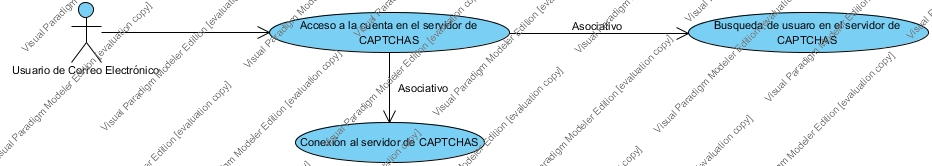
\includegraphics[width=1\linewidth, height=5cm]{./images/casodeuso3.jpg}
	\caption{Diagrama de casos de uso CU3 Acceso a la cuenta en el servidor de CAPTCHAS}
	\label{fig:4-4-1}
\end{figure}
\pagebreak

\subsection{Diagrama de casos de uso CU4 Abrir Correo Electrónico.}
\begin{figure}[H]
	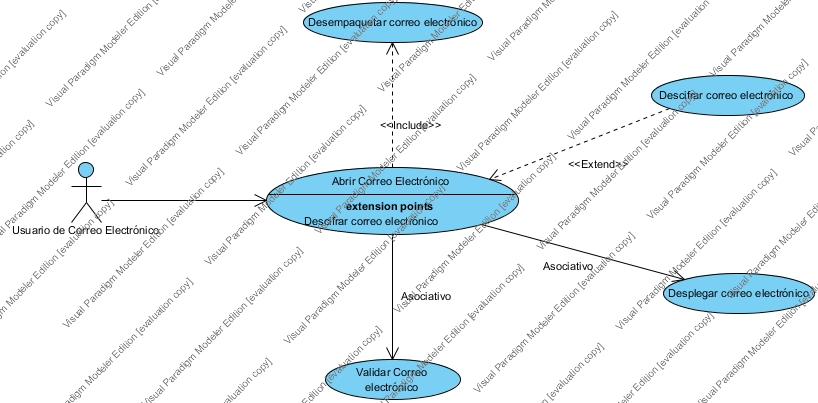
\includegraphics[width=1\linewidth, height=10cm]{./images/casodeuso4.jpg}
	\caption{Diagrama de casos de uso CU4 Abrir Correo Electrónico.}
	\label{fig:4-5-1}
\end{figure}
\begin{table}[H]
\centering
   {
     \begin{tabular}{| p{4,5cm} | p{0,5cm} |p{4cm}|p{5cm}|}
     \hline
     \textbf{Caso de Uso} &\multicolumn{3}{|l|}{CU4 Abrir correo electrónico}\\
     \hline
     \textbf{Actor} & \multicolumn{3}{|l|}{Actor 1. Usuario de correo electrónico}\\
     \hline
     \textbf{Descripción} & \multicolumn{3}{|p{10cm}|}{Describe los pasos necesarios para abrir un mensaje de correo electrónico.}\\
     \hline
     \textbf{Pre-condiciones} & \multicolumn{3}{|p{10cm}|}{1. Iniciar sesión con su servidor de correo electrónico. 2. Descargar el correo electrónico que se desea abrir.}\\
     \hline
     \textbf{Post-condiciones} & \multicolumn{3}{|l|}{Despliegue del mensaje de correo electrónico descifrado.}\\
     \hline
     \textbf{Puntos de inclusión} & \multicolumn{3}{|l|}{Desempaquetar correo electrónico}\\
     \hline
     \textbf{Puntos de extensión} & \multicolumn{3}{|l|}{Descifrar correo electrónico}\\
     \hline
     \textbf{Flujo principal} & & Actor/Sistema & Acción a realizar\\
     \hline
     & 1 & Actor & El caso de uso comienza cuando el usuario selecciona el correo que desea abrir.\\
     \hline
     & 2 & Sistema & El sistema manda a llamar a la función de desempaquetar correo electrónico.\\
     \hline
     & 3 & Sistema & Valida si el mensaje viene timbrado. <FA01 - El mensaje no viene timbrado>\\
     \hline
     & 4 & Sistema & Invoca al caso de uso <CU Descifrar correo electrónico>\\
     \hline
     & 5 & Sistema & Recibe el mensaje de correo electrónico descifrado\\
     \hline
     & 6 & Sistema & Despliega el contenido completo del mensaje al usuario\\
     \hline
     & & & \textbf{Fin del flujo principal}.\\
     \hline
     & \multicolumn{3}{|l|}{\textbf{FA01 - El mensaje no viene timbrado}.}\\
     \hline
     \textbf{Flujo alternativo} & & Actor/Sistema & Acción a realizar\\
     \hline
     & 1 & Sistema & El flujo continúa en el paso 6 del flujo principal.\\
     \hline
     &  & & \textbf{Fin del flujo alternativo}\\
     
     \end{tabular}
    }
    \caption{Descripción CU4.}
    \label{tabla:CU4}
\end{table}


\pagebreak

\subsection{Diagrama casos de uso CU5 Activar cifrado por CAPTCHAS.}
\begin{figure}[H]
	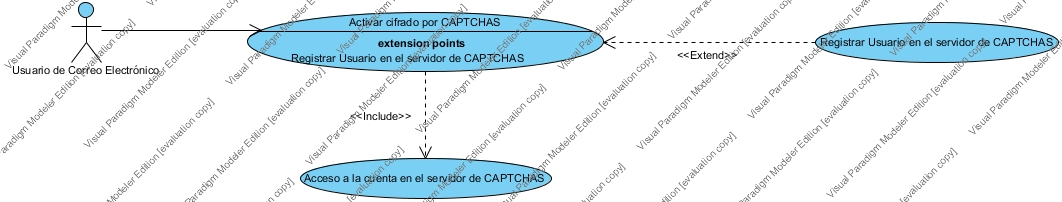
\includegraphics[width=1\linewidth, height=5cm]{./images/casodeuso5.jpg}
	\caption{Diagrama casos de uso CU5 Activar cifrado por CAPTCHAS.}
	\label{fig:4-6-1}
\end{figure}
\begin{longtable}[H]{| p{4,5cm} | p{0,5cm} |p{4cm}|p{5cm}|}
 %\centering
   %{
     %\begin{tabular}
     \hline
     \textbf{Caso de Uso} &\multicolumn{3}{|l|}{CU5 Activar cifrado por CAPTCHAS}\\
     \hline
     \textbf{Actor} & \multicolumn{3}{|l|}{Actor 1. Usuario de correo electrónico}\\
     \hline
     \textbf{Descripción} & \multicolumn{3}{|p{10cm}|}{Describe los pasos necesarios para activar el módulo de cifrado CAPTCHAS en el cliente de correo electrónico.}\\
     \hline
     \textbf{Pre-condiciones} & \multicolumn{3}{|l|}{1. Instalar el módulo de cifrado por CAPTCHAS}\\
     \hline
     \textbf{Post-condiciones} & \multicolumn{3}{|l|}{Activación del cifrado y descifrado por CAPTCHAS.}\\
     \hline
     \textbf{Puntos de inclusión} & \multicolumn{3}{|l|}{}\\
     \hline
     \textbf{Puntos de extensión} & \multicolumn{3}{|l|}{Registrar usuario del servidor de CAPTCHAS}\\
     \hline
     \textbf{Flujo principal} & & Actor/Sistema & Acción a realizar\\
     \hline
     & 1 & Actor & El caso de uso inicia cuando el actor seleccionar la opción "Activar cifrado por CAPTCHAS"\\
     \hline
     & 2 & Sistema & El sistema verifica si la dirección de correo del usuario está registrada en el servidor de CAPTCHAS<FA01 -Usuario no registrado en el servidor>\\
     \hline
     & 3 & Sistema & Despliega una ventana con el mensaje "Activación del módulo de cifrado por CAPTCHAS"\\
     \hline
     & & & \textbf{Fin del flujo principal}.\\
     \hline
     & \multicolumn{3}{|l|}{\textbf{FA01 -Usuario no registrado en el servidor}.}\\
     \hline
     \textbf{Flujo alternativo} & & Actor/Sistema & Acción a realizar\\
     \hline
     & 1 & Sistema & El sistema despliega una ventana con las opciones de "Registrarse" y "Cancelar". <FA02 Cancelar activación>\\
     \hline
     & 2 & Actor & Oprime el botón de "Registrarse"\\
     \hline
     & 3 & Sistema & El sistema invoca al caso de uso <CU Registrar usuario en el servidor de CAPTCHAS>\\
     \hline
     & 4 & Sistema & El sistema obtiene una respuesta satisfactoria del registro\\
     \hline
     & 5 &  & El flujo continúa en el paso 2 del flujo principal.\\
     \hline
     &  & & \textbf{Fin del flujo alternativo}\\
     \hline
     & \multicolumn{3}{|l|}{\textbf{FA02 - Cancelar activación}.}\\
     \hline
     \textbf{Flujo alternativo} & & Actor/Sistema & Acción a realizar\\
     \hline
     & 1 & Actor & El Actor selecciona "Cancelar"\\
     \hline
     & 2 & Sistema & Cierra la ventana de selección\\
     \hline
     & 3 &  & El flujo continúa en el paso 1 del flujo principal.\\
     \hline
     &  & & \textbf{Fin del flujo alternativo}\\
     %\end{tabular}
    %}
    \caption{Descripción CU5.}
    \label{tabla:CU5}
\end{longtable}


\pagebreak
\subsection{Diagrama de casos de uso CU6 Descifrar correo electrónico.}
\begin{figure}[H]
	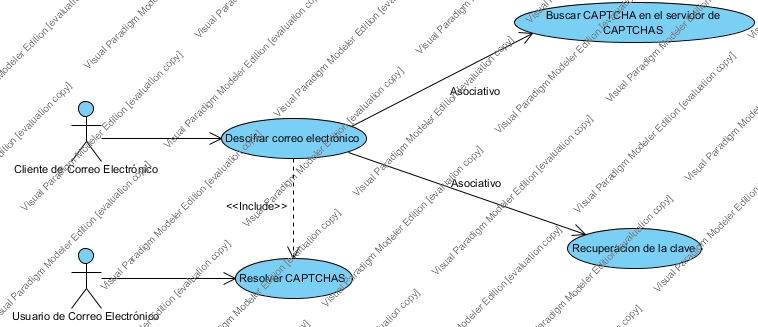
\includegraphics[width=1\linewidth, height=8cm]{./images/casodeuso6.jpg}
	\caption{Diagrama de casos de uso CU6 Descifrar correo electrónico.}
	\label{fig:4-7-1}
\end{figure}
\begin{longtable}[H]{| p{4,5cm} | p{0,5cm} |p{4cm}|p{5cm}|}
 %\centering
   %{
     %\begin{tabular}
     \hline
     \textbf{Caso de Uso} &\multicolumn{3}{|l|}{CU6 Descifrar correo electrónico.}\\
     \hline
     \textbf{Actor} & \multicolumn{3}{|l|}{Actor 1. Usuario de correo electrónico}\\
     \hline
     \textbf{Descripción} & \multicolumn{3}{|p{10cm}|}{Describe los pasos necesarios para desactivar el módulo de cifrado CAPTCHAS en el cliente de correo electrónico}\\
     \hline
     \textbf{Pre-condiciones} & \multicolumn{3}{|p{10cm}|}{1. Activar cifrado por CAPTCHAS. 2. Registrar usuario en el servidor de CAPTCHAS}\\
     \hline
     \textbf{Post-condiciones} & \multicolumn{3}{|l|}{Desactivación del cifrado y descifrado por CAPTCHAS.}\\
     \hline
     \textbf{Puntos de inclusión} & \multicolumn{3}{|l|}{}\\
     \hline
     \textbf{Puntos de extensión} & \multicolumn{3}{|l|}{Eliminar usuario del servidor de CAPTCHAS}\\
     \hline
     \textbf{Flujo principal} & & Actor/Sistema & Acción a realizar\\
     \hline
     & 1 & Actor & El caso de uso inicia cuando el actor seleccionar la opción "Desactivar cifrado por CAPTCHAS"\\
     \hline
     & 2 & Sistema & El sistema despliega la venta con las opciones de "Desactivar cifrado" y "Eliminar usuario" <FA01 - Eliminar usuario>\\
     \hline
     & 3 & Actor & Selecciona la Desactivación del cifrado por CAPTCHAS\\
     \hline
     & 4 & Sistema & El sistema desactiva el módulo de cifrado por CAPTCHA\\
     \hline
     & & & \textbf{Fin del flujo principal}.\\
     \hline
    & \multicolumn{3}{|l|}{\textbf{FA01 - Eliminar usuario}.}\\
    \hline
    \textbf{Flujo alternativo} & & Actor/Sistema & Acción a realizar\\
    \hline
    & 1 & Actor & El Actor selecciona "Eliminar usuario"\\
    \hline
    & 2 & Sistema & El sistema despliega una ventana con las opciones de "Aceptar" y "Cancelar" para confirmar la eliminación del usuario. <FA02 - Cancelar acción eliminar usuario>\\
    \hline
     & 3 & Actor & Oprime el botón de "Aceptar"\\
     \hline
     & 4 & Sistema & Establece la conexión con el servidor de CAPTCHAS <FA03 - Fallo en la conexión con el servidor>\\
     \hline
     & 5 & Sistema & Busca y elimina al usuario de la base de datos desplegando la confirmación del servidor.\\
     \hline
     & 6 & Actor & Oprime el botón de "Aceptar"\\
     \hline
     & 7 & Sistema & Desactiva el módulo de cifrado por CAPTCHA\\
     \hline
     &  & & \textbf{Fin del flujo alternativo}\\
     \hline
     & \multicolumn{3}{|l|}{\textbf{FA02 - Cancelar acción eliminar usuario}.}\\
    \hline
    \textbf{Flujo alternativo} & & Actor/Sistema & Acción a realizar\\
    \hline
    & 1 & Actor & El Actor selecciona "Cancelar"\\
    \hline
    & 2 & Sistema & Cierra la ventana de confirmación\\
    \hline
    &  & & \textbf{Fin del flujo alternativo}\\
     \hline
    & \multicolumn{3}{|l|}{\textbf{FA03 - Fallo en la conexión con el servidor}.}\\
    \hline
    \textbf{Flujo alternativo} & & Actor/Sistema & Acción a realizar\\
    \hline
    & 1 & Sistema & Despliega una ventana de alerta con el mensaje "No se ha podido establecer la conexión con el servidor, es probable que no se tenga conexión a internet. Favor de intentarlo más tarde"\\
    \hline
    & 2 & Actor & Cierra la ventana de alerta\\
    \hline
    & 3 &  & El flujo continúa en el paso 1 del flujo principal\\
    \hline
    &  & & \textbf{Fin del flujo alternativo}\\
    % \end{tabular}
    %}
    \caption{Descripción CU6.}
    \label{tabla:CU6}
\end{longtable}


\pagebreak
\subsection{Diagrama de caos de uso CU7 Eliminar CAPTCHA del servidor.}
\begin{figure}[H]
	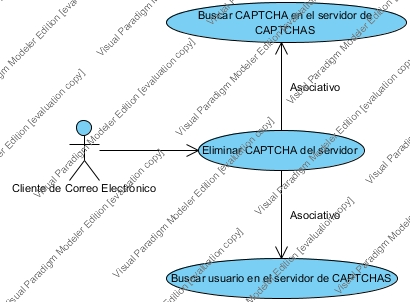
\includegraphics[width=1\linewidth, height=8cm]{./images/casodeuso7.jpg}
	\caption{Diagrama de caos de uso CU7 Eliminar CAPTCHA del servidor.}
	\label{fig:4-8-1}
\end{figure}
\begin{table}[H]
 \centering
   {
     \begin{tabular}{| p{4,5cm} | p{0,5cm} |p{4cm}|p{5cm}|}
     \hline
     \textbf{Caso de Uso} &\multicolumn{3}{|l|}{CU7 Eliminar CAPTCHA del servidor.}\\
     \hline
     \textbf{Actor} & \multicolumn{3}{|l|}{Actor 1. Cliente de correo electrónico.}\\
     \hline
     \textbf{Descripción} & \multicolumn{3}{|p{10cm}|}{Describe los pasos necesarios para eliminar los CAPTCHAS del servidor de CAPTCHAS.}\\
     \hline
     \textbf{Pre-condiciones} & \multicolumn{3}{|l|}{1. Solicitar eliminar un mensaje de correo electrónico}\\
     \hline
     \textbf{Post-condiciones} & \multicolumn{3}{|l|}{}\\
     \hline
     \textbf{Puntos de inclusión} & \multicolumn{3}{|l|}{}\\
     \hline
     \textbf{Puntos de extensión} & \multicolumn{3}{|l|}{}\\
     \hline
     \textbf{Flujo principal} & & Actor/Sistema & Acción a realizar\\
     \hline
     & 1 & Actor & Solicita eliminar CAPTCHA del servidor de CAPTCHAS\\
     \hline
     & 2 & Sistema & Busca al usuario y el CAPTCHA a eliminar en el servidor de CAPTCHAS\\
     \hline
     & 3 & Sistema & Elimina el CAPTCHA solicitado\\
     \hline
     & 4 & Sistema & Regresa la confirmación de que se eliminó el CAPTCHA.\\
     \hline
     & & & \textbf{Fin del flujo principal}.\\
          
     \end{tabular}
    }
    \caption{Descripción CU7.}
    \label{tabla:CU7}
\end{table}


\pagebreak

\subsection{Diagrama de casos de uso CU8 Eliminar correo electrónico.}
\begin{figure}[H]
	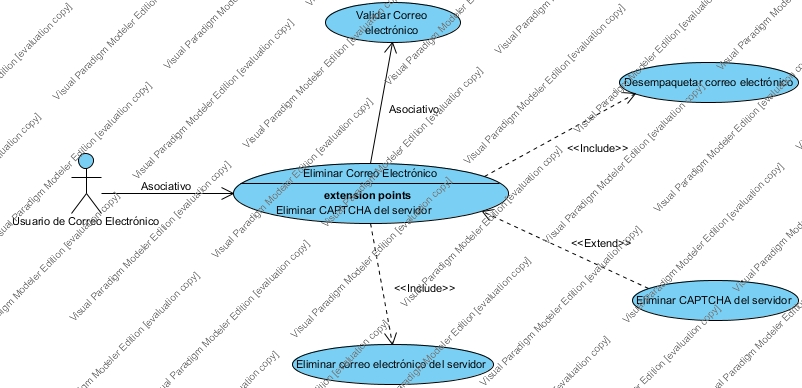
\includegraphics[width=1\linewidth, height=8cm]{./images/casodeuso8.jpg}
	\caption{Diagrama de casos de uso CU8 Eliminar correo electrónico.}
	\label{fig:4-9-1}
\end{figure}
\begin{table}[H]
 \centering
   {
     \begin{tabular}{| p{4,5cm} | p{0,5cm} |p{4cm}|p{5cm}|}
     \hline
     \textbf{Caso de Uso} &\multicolumn{3}{|l|}{CU8 Eliminar correo electrónico.}\\
     \hline
     \textbf{Actor} & \multicolumn{3}{|l|}{Actor 1. Usuario de correo electrónico.}\\
     \hline
     \textbf{Descripción} & \multicolumn{3}{|p{10cm}|}{Describe los pasos necesarios para eliminar un mensaje de correo electrónico.}\\
     \hline
     \textbf{Pre-condiciones} & \multicolumn{3}{|l|}{1. Seleccionar un mensaje de correo electrónico}\\
     \hline
     \textbf{Post-condiciones} & \multicolumn{3}{|l|}{Mensaje y CAPTCHA eliminados.}\\
     \hline
     \textbf{Puntos de inclusión} & \multicolumn{3}{|p{10cm}|}{1. Desempaquetar correo electrónico. 2. Eliminar correo electrónico del servidor}\\
     \hline
     \textbf{Puntos de extensión} & \multicolumn{3}{|l|}{Eliminar CAPTCHA del servidor de CAPTCHAS}\\
     \hline
     \textbf{Flujo principal} & & Actor/Sistema & Acción a realizar\\
     \hline
     & 1 & Actor & Selecciona un mensaje de correo electrónico a eliminar.\\
     \hline
     & 2 & Sistema & Desempaqueta el mensaje de correo electrónico\\
     \hline
     & 3 & Sistema & Valida si el mensaje esta timbrado. <FA01 - Mensaje no timbrado>\\
     \hline
     & 4 & Sistema & Invoca al caso de uso <CU Eliminar CAPTCHA del servidor>\\
     \hline
     & 5 & Sistema & Elimina el mensaje de correo electrónico y despliega el mensaje "El correo se ha eliminado correctamente"\\
     \hline
     & & & \textbf{Fin del flujo principal}.\\
     \hline
     & \multicolumn{3}{|l|}{\textbf{FA01 - Mensaje no timbrado}.}\\
     \hline
     \textbf{Flujo alternativo} & & Actor/Sistema & Acción a realizar\\
     \hline
     & 1 & Sistema & El sistema continúa a partir del paso 5 del flujo principal.\\
     \hline
     &  & & \textbf{Fin del flujo alternativo}\\
     
     \end{tabular}
    }
    \caption{Descripción CU8.}
    \label{tabla:CU8}
\end{table}


\pagebreak
\subsection{Diagrama de casos de uso CU9 Enviar CAPTCHAS}
\begin{figure}[H]
	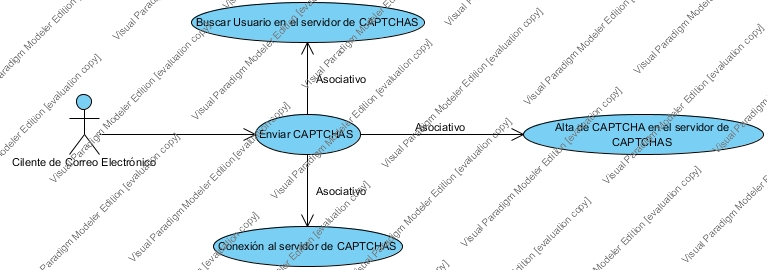
\includegraphics[width=1\linewidth, height=8cm]{./images/casodeuso9.jpg}
	\caption{Diagrama de casos de uso CU9 Enviar CAPTCHAS}
	\label{fig:4-10-1}
\end{figure}

\begin{table}[H]
 \centering
   {
     \begin{tabular}{| p{4,5cm} | p{0,5cm} |p{4cm}|p{5cm}|}
     \hline
     \textbf{Caso de Uso} &\multicolumn{3}{|l|}{CU9 Enviar CAPTCHAS}\\
     \hline
     \textbf{Actor} & \multicolumn{3}{|l|}{Actor 1. Cliente de correo electrónico.}\\
     \hline
     \textbf{Descripción} & \multicolumn{3}{|p{10cm}|}{Describe los pasos necesarios para enviar el CAPTCHA el servidor de CAPTCHAS}\\
     \hline
     \textbf{Pre-condiciones} & \multicolumn{3}{|l|}{1. Solicitar el envió de un nuevo mensaje de correo electrónico.}\\
     \hline
     \textbf{Post-condiciones} & \multicolumn{3}{|l|}{Envío del CAPTCHA al servidor de CAPTCHAS}\\
     \hline
     \textbf{Puntos de inclusión} & \multicolumn{3}{|l|}{}\\
     \hline
     \textbf{Puntos de extensión} & \multicolumn{3}{|l|}{}\\
     \hline
     \textbf{Flujo principal} & & Actor/Sistema & Acción a realizar\\
     \hline
     & 1 & Actor & Solicita el envío de CAPTCHA al servidor\\
     \hline
     & 2 & Sistema & Abre la conexión y busca al usuario en el servidor de CAPTCHAS\\
     \hline
     & 3 & Sistema & Da de alta el CAPTCHA en el servidor asociándolo con el usuario.\\
     \hline
     & 4 & Sistema & Regresa la confirmación de que se dio de alta el CAPTCHA\\
     \hline
     & & & \textbf{Fin del flujo principal}.\\
         
     \end{tabular}
    }
    \caption{Descripción CU9.}
    \label{tabla:CU9}
\end{table}


\pagebreak
\subsection{Diagrama de casos de uso CU10 Enviar correo electrónico.}
\begin{figure}[H]
	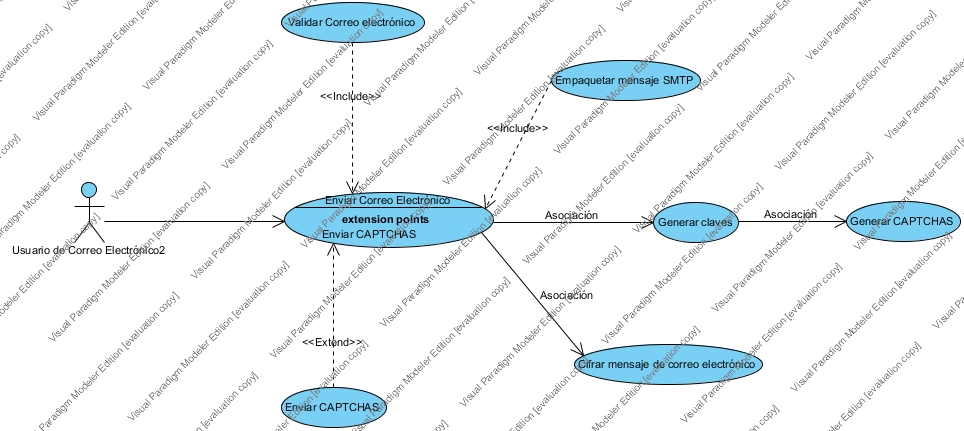
\includegraphics[width=1\linewidth, height=8cm]{./images/casodeuso10.jpg}
	\caption{Diagrama de casos de uso CU10 Enviar correo electrónico.}
	\label{fig:4-11-1}
\end{figure}
\begin{table}[H]
 \centering
   {
     \begin{tabular}{| p{4,5cm} | p{0,5cm} |p{4cm}|p{5cm}|}
     \hline
     \textbf{Caso de Uso} &\multicolumn{3}{|l|}{CU10 Enviar correo electrónico.}\\
     \hline
     \textbf{Actor} & \multicolumn{3}{|l|}{Actor 1. Usuario de correo electrónico.}\\
     \hline
     \textbf{Descripción} & \multicolumn{3}{|p{10cm}|}{Describe los pasos necesarios para enviar un mensaje de correo electrónico cifrado a otro usuario de correo electrónico.}\\
     \hline
     \textbf{Pre-condiciones} & \multicolumn{3}{|p{10cm}|}{1. El usuario tiene que redactar un mensaje de correo electrónico que contenga la dirección del destinatario.}\\
     \hline
     \textbf{Post-condiciones} & \multicolumn{3}{|p{10cm}|}{Envió de un mensaje cifrado al servidor de correo electrónico y el registro del CAPTCHA en el servidor de CAPTCHAS.}\\
     \hline
     \textbf{Puntos de inclusión} & \multicolumn{3}{|p{10cm}|}{1. Validar correo electrónico. 2. Empaquetar mensaje de correo electrónico SMTP.}\\
     \hline
     \textbf{Puntos de extensión} & \multicolumn{3}{|l|}{Enviar CAPTCHA}\\
     \hline
     \textbf{Flujo principal} & & Actor/Sistema & Acción a realizar\\
     \hline
     & 1 & Actor & Oprime el botón "Enviar"\\
     \hline
     & 2 & Sistema & Valida que el mensaje de correo electrónico contenga los datos mínimos.<FA01 - Campos no completados>\\
     \hline
     & 3 & Sistema & Genera una llave de cifrado\\
     \hline
     & 4 & Sistema & Con una palabra aleatoria se genera el CAPTCHA y cifra el mensaje de correo electrónico.\\
     \hline
     & 5 & Sistema & Toma el mensaje cifrado y es empaquetado para enviarse al servidor de correo electrónico\\
     \hline
     & 6 & Sistema & Toma el CAPTCHA  y se envía al caso de uso <CU Enviar CAPTCHA>\\
     \hline
     & 7 & Sistema & Despliega el mensaje de "envío satisfactorio"\\
     \hline
     & & & \textbf{Fin del flujo principal}.\\
     \hline
     & \multicolumn{3}{|l|}{\textbf{FA01 - Campos no completados}.}\\
     \hline
     \textbf{Flujo alternativo} & & Actor/Sistema & Acción a realizar\\
     \hline
     & 1 & Sistema & Notifica al usuario cuales campos han sido mal proporcionados, para poder enviar el mensaje correctamente\\
     \hline
     & 2 & Actor & Modifica los campos solicitados\\
     \hline
     & 3 &  & El flujo continúa en el paso 1 del flujo principal\\
     \hline
     &  & & \textbf{Fin del flujo alternativo}\\
     
     \end{tabular}
    }
    \caption{Descripción CU10.}
    \label{tabla:CU10}
\end{table}



\pagebreak
\section{Diagramas a bloques}
A continuación se presentan los diagramas a bloques, en donde se muestra cuál es la secuencia de procesos a realizar. Esto servirá para comprender cómo se comunican los diferentes módulos de manera interna, y cómo hacen los procesos.


\begin{figure}[H]
	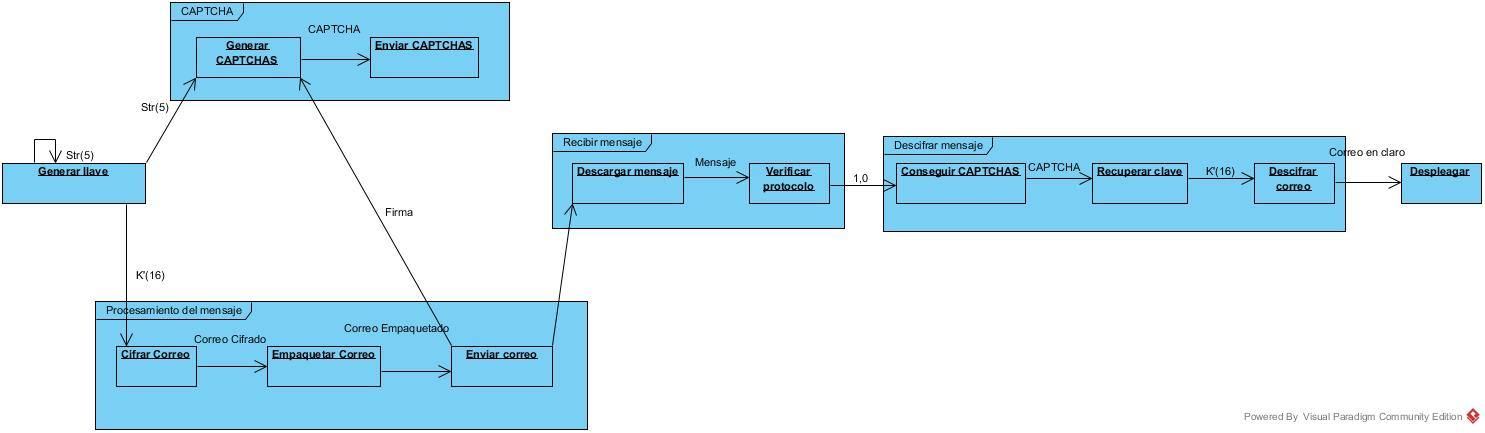
\includegraphics[width=1\linewidth, height=5cm]{./images/bloques0.jpg}
	\caption{Diagrama a bloque 0 general del sistema}
	\label{fig:5-1-1}
\end{figure}
\pagebreak
\begin{table}[H]
 \centering
   {
     \begin{tabular}{| p{2,2cm} | p{1,7cm} | p{2,5cm} | p{3cm} | p{2cm} | p{2,1cm} | p{2cm} |}
     \hline
     & \textbf{Generar clave} & \textbf{Generar CAPTCHA} & \textbf{Procesamiento del mensaje} & \textbf{Recibir mensaje} & \textbf{Descifrar mensaje} & \textbf{Desplegar}\\
     \hline
     \textbf{Entradas} & *Señal de activación & *Cadena de 5 caracteres: Str(5) & *Clave de 16 bytes: K’(16). *Mensaje de correo. & *Correo Cifrado & Verificación (1,0) & *Correo en claro\\
     \hline
     \textbf{Salidas} & *Cadena de 5 caracteres: Str(5) *Clave de 16 bytes: K’(16) & *Señal de envió & *Correo Cifrado & *Verificación (1,0) & *Correo en claro&\\
     \hline
     \textbf{Descripción} & Se activa el proceso generar clave, este crea una palabra de 5 caracteres (Str(5)), procesa la palabra Str(5) por medio de una función hash obteniendo una palabra de 256 caracteres (K(256)) y recorta esta clave a una palabra de 16 caracteres (K’(16)). & Toma la entrada Str(5) y la convierte en una imagen CAPTCHA, Posteriormente inicia una conexión con el servidor de CAPTCHAS para mandarlo a este. & Cifra el mensaje de correo con la clave K’(16), posteriormente lo firma y genera un timbre para saber que fue creado con este esquema y lo empaqueta para su envió. & El cliente hace una petición al servidor y descarga el mensaje de correo electrónico, lo des empaqueta verifica la firma y el timbrado para saber de quién viene y si está cifrado bajo este esquema. & Se hace una petición al servidor de CAPTCHAS, se descargan los CAPTCHAS asociados al correo, ya con el CAPTCHA este se resuelve y se recupera la cadena Str(5), esta se pasa por una función hash y se recupera K(256), esta se corta a K’(16), con esto se descifra el mensaje. & Se muestra el correo descifrado en la interfase del cliente de correo electrónico.\\

    \end{tabular}
    }
    \caption{Diagrama a bloques 0 general}
    \label{tabla:b0}
\end{table}


\newpage
\newpage
%\subsection{Diagrama a bloques 1 Generar clave}
\begin{figure}[H]
	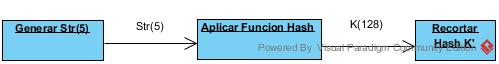
\includegraphics[width=1\linewidth, height=2cm]{./images/bloques1.jpg}
	\caption{Diagrama a bloques 1 Generar clave}
	\label{fig:5-2-1}
\end{figure}
\begin{table}[H]
 \centering
   {
     \begin{tabular}{| p{4cm} | p{4cm} | p{4cm} | p{4cm} |}
     \hline
     & \textbf{Generar Str(5)} & \textbf{Aplicar Función Hash} & \textbf{Recortar Hash K’}\\
     \hline
     \textbf{Entradas} & *Llamada a Función & *Cadena de 5 caracteres: Str(5) & *Digesto K(128)\\
     \hline
     \textbf{Salidas} & *Cadena de 5 caracteres: Str(5) & *Digesto K(128) & *K’(16)\\
     \hline
     \textbf{Descripción} & Toma una función random módulo 67, para formar una palabra con 5 caracteres aleatorios tomados del siguiente conjunto.Anillo67{-.,+*[a-z][A-Z]} & Se pasa la cadena Str(5) por una función hash SHA-1 para obtener un digesto único de esta palabra. & Se copian a otro string lo primeros 16 caracteres del digesto K(128) para formar la clave K’(16)\\

    \end{tabular}
    }
    \caption{Diagrama a bloques 1 general clave}
    \label{tabla:b1}
\end{table}

\begin{table}[H]
 \centering
   {
     \begin{tabular}{| p{3cm} | p{3cm} |}
     \hline
     & \textbf{Cifrar}\\
     \hline
     \textbf{Entradas} & *Clave K’(16) *Mensaje de correo\\
     \hline
     \textbf{Salidas} & *Correo cifrado\\
     \hline
     \textbf{Descripción} & Se cifra el mensaje con un algoritmo de llave simétrica (AES o DES) usando una llave de 16bytes o 128bits.\\

    \end{tabular}
    }
    \caption{Diagrama a bloques 2 Cifrar Correo}
    \label{tabla:b2}
\end{table}

\begin{figure}[H]
	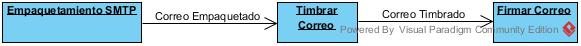
\includegraphics[width=1\linewidth, height=1cm]{./images/bloques3.jpg}
	\caption{Diagrama a bloques 3 Empaquetar Correo}
	\label{fig:5-3-1}
\end{figure}

\begin{table}[H]
 \centering
   {
     \begin{tabular}{| p{4cm} | p{4cm} | p{4cm} |}
     \hline
     & \textbf{Empaquetamiento SMTP} & \textbf{Timbrar Correo}\\
     \hline
     \textbf{Entradas} & *Mensaje Cifrado & *Correo Empaqueta\\
     \hline
     \textbf{Salidas} & *Correo Empaquetado & *Correo Timbrado\\
     \hline
     \textbf{Descripción} & Se toma el correo y se integra en el formato del correo marcado en el RFC822 & Se timbra el mensaje colocando una marca después del final del mensaje. Para señalar que el correo enviado está cifrado bajo este protocolo.\\

    \end{tabular}
    }
    \caption{Diagrama a bloques 3 Empaquetar Correo}
    \label{tabla:b3}
\end{table}

\begin{figure}[H]
	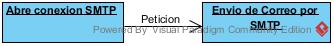
\includegraphics[width=1\linewidth, height=2cm]{./images/bloques4.jpg}
	\caption{Diagrama a bloques 4 Enviar correo}
	\label{fig:5-4-1}
\end{figure}

\begin{table}[H]
 \centering
   {
     \begin{tabular}{| p{4cm} | p{4cm} | p{4cm} |}
     \hline
     & \textbf{Abrir conexión SMTP} & \textbf{Envió de Correo por SMTP}\\
     \hline
     \textbf{Entradas} & *Petición & *Correo empaquetado\\
     \hline
     \textbf{Salidas} & *Canal de comunicación & *Confirmación de envió\\
     \hline
     \textbf{Descripción} & Se genera una petición para conexión SMTP  & Se manda el correo electrónico al servidor por medio del protocolo SMTP\\

    \end{tabular}
    }
    \caption{Diagrama a bloques 4 Enviar correo}
    \label{tabla:b4}
\end{table}
\clearpage
\begin{figure}[H]
	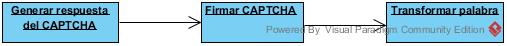
\includegraphics[width=1\linewidth, height=2cm]{./images/bloques5.jpg}
	\caption{Diagrama a bloques 5 Generar CAPTCHA}
	\label{fig:5-5-1}
\end{figure}
\begin{table}[H]
 \centering
   {
     \begin{tabular}{| p{4cm} | p{4cm} | p{4cm} | p{4cm} |}
     \hline
     & \textbf{Generar respuesta del CAPTCHA} & \textbf{Firmar CAPTCHA} & \textbf{Transformar palabra}\\
     \hline
     \textbf{Entradas} & *Cadena de caracteres: Str(5) & *Firma & *Señal de confirmación\\
     \hline
     \textbf{Salidas} & *Señal de confirmación & *Archivo Firmado & *Imagen CAPTCHA\\
     \hline
     \textbf{Descripción} & Genera un archivo con la respuesta del CAPTCHA  & Se firma el CAPTCHA por medio de un Hashing del mensaje. & Convierte el Str(5) en una imagen distorsionada que llamaremos CAPTCHA\\

    \end{tabular}
    }
    \caption{Diagrama a bloques 5 Generar CAPTCHA}
    \label{tabla:b5}
\end{table}
\newpage
\begin{figure}[H]
	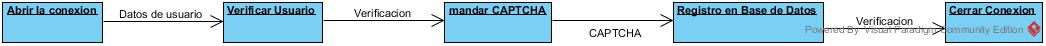
\includegraphics[width=1\linewidth, height=1cm]{./images/bloques6.jpg}
	\caption{Diagrama a bloques 6 Enviar CAPTCHAS (Usuario existente)}
	\label{fig:5-6-1}
\end{figure}

\begin{table}[H]
 \centering
   {
     \begin{tabular}{| p{2,5cm} | p{2,5cm} | p{2,5cm} | p{2,5cm} | p{2,5cm} | p{2,5cm} |}
     \hline
     & \textbf{Abrir conexión} & \textbf{Verificar Usuario} & \textbf{Mandar CAPTCHA} & \textbf{Registrar en base de datos} & \textbf{Cerrar Conexión}\\
     \hline
     \textbf{Entradas} & *CAPTCHAS & *Datos de Usuario & *Verificación de usuario & *Datos de usuario *CAPTCHA & Verificación\\
     \hline
     \textbf{Salidas} & *Datos de usuario & *Verificación de usuario & *CAPTCHA & Verificación &\\
     \hline
     \textbf{Descripción} & Se genera una petición para poder entablar una conexión con el servidor de CAPTCHAS & Se verifica la existencia del usuario en el servidor, si existe se le da acceso & Ya verificado el usuario se manda el CAPTCHA al servidor & Se registran los datos del CAPTCHA en la base de datos y se envía una verificación & Se cierra la conexión y se guardan los datos\\

    \end{tabular}
    }
    \caption{Diagrama a bloques 6 Enviar CAPTCHAS (Usuario existente)}
    \label{tabla:b6}
\end{table}
\pagebreak
\begin{figure}[H]
	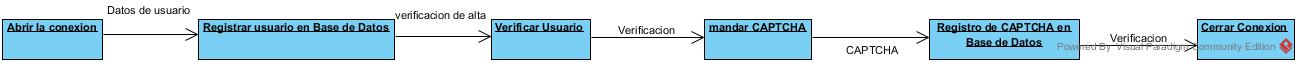
\includegraphics[width=1\linewidth, height=1cm]{./images/bloques7.jpg}
	\caption{Diagrama a bloques 7 Enviar CAPTCHAS (Usuario inexistente)}
	\label{fig:5-7-1}
\end{figure}
\begin{table}[H]
 \centering
   {
     \begin{tabular}{| p{2cm} | p{2cm} | p{2,5cm} | p{2cm} | p{2,5cm} | p{2,5cm} | p{2cm} |}
     \hline
     & \textbf{Abrir conexión} & \textbf{Registrar usuario en Base de Datos} & \textbf{Verificar Usuario} & \textbf{Mandar CAPTCHA} & \textbf{Registrar en base de datos} & \textbf{Cerrar Conexión}\\
     \hline
     \textbf{Entradas} & *CAPTCHAS & *Datos de Usuario & *Verificación de registro & *Verificación de usuario & *Datos de usuario *CAPTCHA & Verificación\\
     \hline
     \textbf{Salidas} & *Datos de usuario & *Verificación de registro & *Verificación de usuario & *CAPTCHA & Verificación &\\
     \hline
     \textbf{Descripción} & Se genera una petición para poder entablar una conexión con el servidor de CAPTCHAS & Se da de alta al usuario en la base de datos & se le da acceso  al usuario & Ya verificado el usuario se manda el CAPTCHA al servidor & Se registran los datos del CAPTCHA en la base de datos y se envía una verificación & Se cierra la conexión y se guardan los datos\\

    \end{tabular}
    }
    \caption{Diagrama a bloques 7 Enviar CAPTCHAS (Usuario inexistente)}
    \label{tabla:b7}
\end{table}
\pagebreak
\begin{figure}[H]
	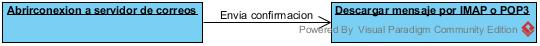
\includegraphics[width=1\linewidth, height=1cm]{./images/bloques8.jpg}
	\caption{Diagrama a bloques 8 Descargar mensaje}
	\label{fig:5-8-1}
\end{figure}
\begin{table}[H]
 \centering
   {
     \begin{tabular}{| p{3cm} | p{4cm} | p{4cm} |}
     \hline
     & \textbf{Abrir conexión al servidor de correo} & \textbf{Descargar mensaje por IMAP o POP3}\\
     \hline
     \textbf{Entradas} & *Señal de activación & *Confirmación\\
     \hline
     \textbf{Salidas} & *Confirmación & *Correo electrónico\\
     \hline
     \textbf{Descripción} & El receptor se conecta al servidor de correo electrónico e inicia la sesión & Descarga del servidor de correo electrónico todos los mensajes que aún no se hayan descargado.\\

    \end{tabular}
    }
    \caption{Diagrama a bloques 8 Descargar mensaje}
    \label{tabla:b8}
\end{table}
\begin{figure}[H]
	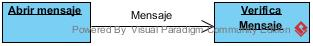
\includegraphics[width=1\linewidth, height=1cm]{./images/bloques9.jpg}
	\caption{Diagrama a bloques 9 Verificar protocolo (con protocolo valido)}
	\label{fig:5-9-1}
\end{figure}
\begin{table}[H]
 \centering
   {
     \begin{tabular}{| p{3cm} | p{4cm} | p{4cm} |}
     \hline
     & \textbf{Abrir mensaje} & \textbf{Verificar mensaje}\\
     \hline
     \textbf{Entradas} & *Correo electrónico & *mensaje\\
     \hline
     \textbf{Salidas} & *Mensaje & *verificación\\
     \hline
     \textbf{Descripción} & Se toma el mensaje descargado del servidor y se des empaqueta para dejar solo el texto del mensaje & Se verifica que el mensaje tenga la bandera correspondiente a que está cifrado con este esquema\\

    \end{tabular}
    }
    \caption{Diagrama a bloques 9 Verificar protocolo (con protocolo válido)}
    \label{tabla:b9}
\end{table}


\clearpage
\begin{table}[H]
 \centering
   {
     \begin{tabular}{| p{3cm} | p{4cm} | p{4cm} |}
     \hline
     & \textbf{Abrir mensaje} & \textbf{Verificar mensaje}\\
     \hline
     \textbf{Entradas} & *Correo electrónico & *mensaje\\
     \hline
     \textbf{Salidas} & *Mensaje & *verificación\\
     \hline
     \textbf{Descripción} & Se toma el mensaje descargado del servidor y se des empaqueta para dejar solo el texto del mensaje & Si la verificación es negativa se manda directamente al bloque de Despliegue\\

    \end{tabular}
    }
    \caption{Diagrama a bloques 10 Verificar protocolo (con protocolo inválido)	}
    \label{tabla:b10}
\end{table}

\begin{figure}[H]
	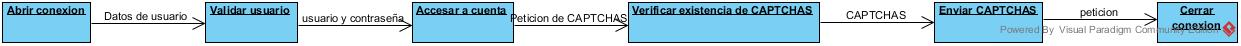
\includegraphics[width=1\linewidth, height=1cm]{./images/bloques11.jpg}
	\caption{Diagrama a bloques 11 Conseguir CAPTCHAS (Usuario existente)}
	\label{fig:5-11-1}
\end{figure}
\begin{table}[H]
 \centering
   {
     \begin{tabular}{| p{2,5cm} | p{3cm} | p{2cm} | p{2cm} | p{3cm} | p{3cm} |}
     \hline
     & \textbf{Abrir Conexión} & \textbf{Validar Usuario} & \textbf{Accesar a cuenta} & \textbf{Verificar existencia de CAPTCHA} & \textbf{Enviar CAPTCHA}\\
     \hline
     \textbf{Entradas} & *Confirmación & *Datos usuario & *Contraseña & *Petición de CAPTCHAS & *Confirmación\\
     \hline
     \textbf{Salidas} & *verificación & *Contraseña & *confirmación & *confirmación & *CAPTCHA\\
     \hline
     \textbf{Descripción} & Se abre una conexión con el servidor de CAPTCHAS & Se verifica que el usuario este dado de alta en el servidor mandándole una petición a la base de datos, si el usuario existe se accesa & Si esta dado de alta en el servidor se manda la contraseña para que pueda tener acceso a los CAPTCHAS de su cuenta & Se verifica que los CAPTCHAS que están ligados al mensaje que realizo la petición existan & Si existen estos CAPTCHAS son enviados de regreso al mensaje\\

    \end{tabular}
    }
    \caption{Diagrama a bloques 11 Conseguir CAPTCHAS (Usuario existente)}
    \label{tabla:b11}
\end{table}

\begin{figure}[H]
	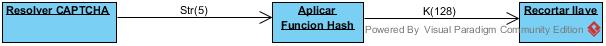
\includegraphics[width=1\linewidth, height=1cm]{./images/bloques12.jpg}
	\caption{Diagrama a bloques 12 Recuperar clave}
	\label{fig:5-12-1}
\end{figure}
\begin{table}[H]
 \centering
   {
     \begin{tabular}{| p{2,5cm} | p{3cm} | p{3cm} | p{3cm} |}
     \hline
     & \textbf{Resolver CAPTCHA} & \textbf{Aplicar Función Hash} & \textbf{Recortar llave}\\
     \hline
     \textbf{Entradas} & *CAPTCHA & *Cadena de 5 caracteres: Str(5) & *Digesto K(128)\\
     \hline
     \textbf{Salidas} & *Str(5) & *Digesto K(128) & *K’(16)\\
     \hline
     \textbf{Descripción} & Se despliega el CAPTCHA para que el usuario pueda resolverlo & Se pasa la cadena Str(5) por una función hash SHA-1 para obtener un digesto único de esta palabra & Se copian a otro string lo primeros 16 caracteres del digesto K(128) para formar la clave K’(16)\\

    \end{tabular}
    }
    \caption{Diagrama a bloques 12 Recuperar clave}
    \label{tabla:b12}
\end{table}
\begin{table}[H]
 \centering
   {
     \begin{tabular}{| p{2,5cm} | p{3cm} |}
     \hline
     & \textbf{Descifrar}\\
     \hline
     \textbf{Entradas} & *Clave K’(16) *Mensaje de correo\\
     \hline
     \textbf{Salidas} & *Correo descifrado\\
     \hline
     \textbf{Descripción} & Se descifra el mensaje con un algoritmo de llave simétrica (AES o DES) usando una llave de 16bytes o 128bits.\\

    \end{tabular}
    }
    \caption{Diagrama a bloques 13 Descifrar correo}
    \label{tabla:b13}
\end{table}

\chapter{Desarrollo de prototipos}
\textbf{Objetivo del prototipo}:
Conocer el uso, funcionamiento e implementación de herramientas de cifrado, hashing y generación de CAPTCHAS, con el fin de conocer la integración de estos módulos en diferentes lenguajes de programación.\\
\section{Prototipo 1}
Se implementó un módulo de cifrado de mensajes de texto en lenguaje C++. Tratando de simular el proceso de cifrado del esquema que se esta usando.\\
La primera parte del proceso es abrir el mensaje para lo cual se estan usando los metodos estandar definidos en las bibliotecas nativas de C++, posteriormente se generara una palabra aleatoria de 5 caracteres usando una función Rand()\%100 y transformando el valor de salida a un char.\\
Al resultado se pasa por una función de hashing, esta función no es nativa de ninguna biblioteca estándar de C++ ni de C, por lo que se tuvo que conseguir una en internet y probar que efectivamente funcionara como lo necesitamos.\\
Posteriormente este hash se usara como llave para cifrar el mensaje que ya abrimos, para esto necesitaremos una función AES o DES, ninguna de estas es estándar de alguna biblioteca de C o C++, así que tendremos que buscarlas y verificar su funcionamiento.\\


\textbf{Conclusión}:
Podemos ver que en C++ el proceso es simple pero se necesita buscar muy bien las bibliotecas externas que se usaran, ya que no siempre están funcionando correctamente, en algunos casos están ni siquiera compilan.\\
Este caso fue particularmente evidente al buscar una biblioteca de C o C++ que pudiera realizar el cifrado con AES o DES, encontrándonos con bibliotecas que cifraban mal ya que al meter la misma llave no descifraban e incluso bibliotecas que no logramos hacer que compilaran.\\

\section{Prototipo 2}
Se implementó un módulo de cifrado, descifrado y generación de CAPTCHAS en Python, simulando el proceso antes del envío del correo y el que se hace después de la recepción de los correos electrónicos.\\
Para este se usó el formato estándar del correo electrónico especificado en el RFC 822, también se usaron bibliotecas ya estandarizadas de python para la implementación de las funciones de hashing, funciones de cifrado y descifrado (AES o DES), funciones aleatorias y la generación de los CAPTCHAS.\\


\textbf{Conclusión}:
Se logró generar todo el proceso de envío y parte del proceso de recepción de mensajes. En cuanto a el envió se logró leer el mensaje, crear una palabra a partir de funciones random, crear la llave con esa string y cifrar el correo exitosamente, además de esto se logró leer el archivo de mensaje de correo electrónico y cifrar únicamente el mensaje que viene en este.\\
Por su parte el módulo de generación de CAPTCHAS mostró muchos problemas para generarlos, ya que no logramos hacer que el intérprete pudiera encontrar correctamente las funciones de la biblioteca de generación CAPTCHAS por lo que al no poder generar un CAPTCHA la recuperación no se puede realizar como se planteó, para verificar únicamente que las funciones sirven se implementó el descifrado del mensaje en el mismo método.\\


\textbf{Objetivo}
Generar una imagen un CAPTCHA a partir de una cadena de caracteres ingresada desde una interfaz gráfica.
\section{Prototipo 3}
Este prototipo se construyó en 2 partes; la primera parte fue la interfaz gráfica y sus herramientas, y la segunda en las herramientas para generar la imagen a partir de una cadena de caracteres.\\
Para la interfaz gráfica se utilizaron las siguientes herramientas para desarrollar este prototipo:\\
Biblioteca Qt y Qt creator: Utilizamos esta biblioteca para generar la interfaz gráfica con la que ingresara la cadena de caracteres y el IDE Qt Creator para facilitar la gestión de las clases.\\
La interfaz gráfica consta de un apartado para ingresar la cadena de caracteres y un botón para convertir la cadena a una imagen de CAPTCHAS.\\
Para generar CAPTCHAS se utilizaron las siguientes herramientas:\\
Lenguaje PHP: se utilizó para genera las imágenes CAPTCHAS con la cadena de caracteres proporcionada anteriormente.\\
En un principio se buscó una biblioteca que generara las imágenes CAPTCHAS en el lenguaje C++ pero su implementación no estaba optimizada y necesitaba ser adaptada casi en su totalidad que tener el funcionamiento deseado, por esta razón buscamos otra biblioteca que se adaptara más a la funcionalidad del prototipo, por lo tanto se optó por utilizar el lenguaje PHP ya que tiene librerías optimizadas para generar imágenes CAPTCHAS.\\
\textbf{Conclusión.}
La generación de imágenes CAPTCHAS es rápida y fácil de implementar, pero durante la investigación nos dimos cuenta que el cliente de correo “Thunderbird” está desarrollado en el lenguaje de programación Python y al no tener una biblioteca nativa en el lenguaje C++ para convertir una cadena de caracteres en CAPTCHAS y  decidimos cambiar de lenguaje de programación.\\


\textbf{Objetivo del prototipo.}
Instalar y configurar un servidor de correo electrónico para el envío de mensajes de correo electrónico entre diferentes usuarios.\\
\section{Prototipo 4}
Instalación y configuración de un servidor de correo electrónico y un servidor DNS.\\


Para el desarrollo de este prototipo fue necesario instalar el servidor de correo electrónico con el protocolo pop y imap, un cliente de correo electrónico web, un servidor DNS y el servidor HTTP Apache. Estos 3 servicios fueron levantados en una computadora con un sistema operativo Xubuntu 15.04; primero se instaló el servidor HTTP\cite{HTTP}, posteriormente pasamos a instalar el servidor DNS y configurar un dominio\cite{DNS}; seguimos con la instalación del servidor de correo electrónico y los protocolos pop y imap; y por último se instaló y  configuro el cliente de correo web\cite{web}.\\
Para la instalación de servidor HTTP fue necesario seguir los siguientes pasos:\
\begin{itemize}
 \item Abrimos una terminar en Ubuntu y escribimos el comando: “sudo apt-get install apache2”
 \item Abrimos como administrador el archivo /etc/apache2/sites-enabled/00-default.conf y escribimos la siguiente configuración:
 \begin{lstlisting}[frame=single]
  <VirtualHost *:80>
     ServerAdmin nombredelsitio@example.com
     ServerName nombredelsitio
     ServerAlias www.nombredelsitio.com
     DocumentRoot /var/www/nombredelsitio.com/public_html/
     ErrorLog /var/www/nombredelsitio.com/logs/error.log
     CustomLog /var/www/nombredelsitio.com/logs/access.log combined
</VirtualHost>
 \end{lstlisting}
 \item Levantamos el servicio http con el siguiente comando: “sudo service apahce2 start”
 \item Para verificar la instalación abrimos un explorador y escribirlos en la barra de búsqueda la siguiente dirección: http://localhost/ y nos aparecerá la siguiente pantalla.
\end{itemize}


Una vez instalado el servidor HTTP proseguimos a instalar el servidor DNS, para levantar este servicio es necesario seguir los siguientes pasos:
\begin{itemize}
 \item Seleccionamos un nombre de dominio, para fines prácticos nuestro dominio privado será “correocifrado.edu”.
 \item Abrimos una terminar en Ubuntu y escribimos el siguiente comando: “sudo apt-get install bind9”
 \item Realizar una copia de respaldo del archivo de configuración original con el comando “cp /etc/bind/named.conf.local \\ /etc/bind/named.conf.local.original”
 \item Editamos el archivo de configuración con: “nano /etc/bind/named.conf.local”
 \item Agregamos al final del archivo lo siguiente:
 \begin{lstlisting}[frame=single]
  zone "correocifrado.edu" {
  type master;
  file "correocifrado.edu.zone";
  };

  zone "10.168.192.in-addr.arpa" {
  type master;
  file "db.192.168.10";
  };
 \end{lstlisting}
 \item Procedamos a crear los (nuevos) archivos de zona, esos archivos contienen los registros del DNS y en Ubuntu se encuentran en el directorio /var/cache/bind/ “nano /var/cache/bind/db.isti.edu.ni.zone”
 \item En el archivo agregamos el siguiente texto:
 \begin{lstlisting}[frame=single]
  $ORIGIN correocifrado.edu.
$TTL 86400            ; 1 dia
@       IN      SOA ns.correocifrado.edu. info.correocifrado.edu. (
        2014112401    ; serie
        6H            ; refresco (6 horas)
        1H            ; reintentos (1 hora)
        2W            ; expira (2 semanas)
        3H            ; mínimo (3 horas)
)

@      IN       NS     ns
@      IN       MX 10  mail
ns     IN       A      192.168.10.10
mail   IN       A      192.168.10.10
www    IN       A      192.168.10.10
 \end{lstlisting}
 \item De igual manera el archivo de zona de búsqueda inversa:\\
  nano /var/cache/bind/db.192.168.10
  \item Agregamos la siguiente configuración:    
  \begin{lstlisting}[frame=single]
   $ORIGIN 10.168.192.in-addr.arpa.
$TTL 86400     ; 1 dia
@       IN  SOA ns.correocifrado.edu. info.correocifrado.edu. (
        2014112401    ; serie
        6H            ; refresco (6 horas)
        1H            ; reintentos (1 hora)
        2W            ; expira (2 semanas)
        3H            ; mínimo (3 horas)
)

@       IN      NS     correocifrado.edu.
10      IN      PTR     correocifrado.edu.
10      IN      PTR     mail.correocifrado.edu.
10      IN      PTR     www.correocifrado.edu.
  \end{lstlisting}
  \item Procedemos a re-iniciar el servicio con el comando “service bind9 restart”
  \item Cambiar el primero de los servidores DNS por la IP del nuestro: “nameserver 192.168.10.10”
  \item Lo único que quede es realizar las pruebas en el cliente “nslookup www.correocifrado.edu”
\end{itemize}
Seguimos con la instalación del servidor de correo electrónico y los servicios del protocolo pop y imap con la aplicación courier-pop y courier-imap:
\begin{itemize}
 \item Abrimos una terminal y escribimos el siguiente comando: “sudo apt-get install postfix”
 \item Durante la instalación nos aparecerá una pantalla de configuración, damos enter para aceptar la configuración.
 \item En tipo genérico de configuración de correo seleccionaremos "Sitio de Internet".
 \item A continuación indicaremos el nombre de sistema de correo, normalmente la dirección del dominio registrado, en nuestro caso "cifradocorreo.net".
 \item Con esto veremos que postfix terminara de instalarse y procedemos a editar el archivo “/etc/postfix/main.cf”.
 \item Añadiremos al final del fichero main.cf las líneas:
 \begin{lstlisting}[frame=single]
  inet_protocols = ipv4
home_mailbox = emails/
 \end{lstlisting}
 \item Una vez guardado el archivo que editamos procedemos a reiniciar el servidor con el comando “sudo /etc/init.d/posrfix restart”
\end{itemize}


Una vez instalado el servicio de correo electrónico procedemos a instalar el courier-pop y el courier-imap.
\begin{itemize}
 \item Abrimos una terminal el Ubuntu y escribimos el siguiente comando “sudo apt-get install courier-pop”.
 \item Nos mostrará una ventana de configuración de courier-base, seleccionamos “NO”.
 \item Procedemos a instalar courier-imap con el siguiente comando “sudo apt-get install courier-imap”.
 \item Esperamos a que finalice la instalación.
\end{itemize}


Por ultimo necesitamos instalar una aplicación webmail para enviar correos entre usuarios del correo electrónico.
\begin{itemize}
 \item Abrimos una terminar en Ubuntu y escribimos el siguiente comando “sudo apt-get install squirrelmail”.
 \item Tras la instalación de SquirrelMail lo configuraremos ejecutando el siguiente comando “sudo squirrelmail-configure”
 \item Selecciónanos la letra D y damos enter.
 \item En este nuevo menú tecleamos la opción courier y damos enter.
 \item Nos dará un informe de la configuración que seleccionamos y damos enter para continuar.
 \item Regresamos al primer menú, ahora tecleamos el número 2 y damos enter.
 \item Seleccionamos en este nuevo menú la opción 1 y damos enter nuevamente.
 \item Nos pedirá nuestro nombre de dominio, en nuestro caso es el dominio que configuramos en el servidor DNS “correocifrado.net”
 \item Nos regresara al menú principal y tecleamos la letra Q para salir de la configuración.
 \item Preguntara si queremos guardar los cambios y tecleamos la letra Y.
 \item Por ultimo ejecutamos el siguiente comando para levantar SquirrelMail en Apache “sudo ln -s /usr/share/squirrelmail /var/www/webmail”
 \item Reiniciamos el servicio apache con el comando “sudo service restart apache2”.
 \item Ya podremos entrar a la aplicación escribiendo el explorador “www.correocifrado.edu/webmail”
\end{itemize}


Para poder enviar correos se necesitan usuarios que desean enviar mensajes entre usuarios, primero crearemos un usuario
\begin{itemize}
 \item Abrimos una terminal de Ubuntu y escribimos el siguiente comando “sudo adduser nombreusuario”.
 \item Introduzca la nueva contraseña de UNIX: introduciremos la contraseña para el usuario, es importante que sea segura (números, letras, mayúsculas y minúsculas) pues con el usuario y la contraseña podremos acceder vía web al servidor de correo electrónico desde cualquier parte del mundo.
 \item Vuelva a escribir la nueva contraseña de UNIX: repetiremos la contraseña.
 \item Full Name: introduciremos el nombre completo, por ejemplo "Alicia Robles Maldonado".
 \item Room Number: Número de oficina.
 \item Work Phone: teléfono del trabajo.
 \item Home Phone: teléfono particular.
 \item Other: otros datos del usuario.
 \item Respondemos "S" a la pregunta "¿Es correcta la información?". Y ya tendremos el usuario creado en el sistema operativo, que también servirá como usuario (buzón) para el servidor de mail.
 \item Ahora generamos el buzón con el siguiente comando “sudo maildirmake /home/nombreusuario/emails”
 \item Cambiamos los permisos de las carpeta emails con el comando “sudo chdown nombreusuario:nombreusuario /home/nombreusuario/emails -R
\end{itemize}
Para crear otro usuario es necesario repetir los pasos anteriores.

\bibliographystyle{IEEEannot}
\begin{thebibliography}{a}
\bibitem{@}
   \textsc{Email}, Internet: \url{http://en.wikipedia.org/wiki/Email}, Mayo, 2015
 \bibitem{sp}
   \textsc{Interactive Advertising Bureau}, Marcelo Brodsky, “Reflexiones jurídicas sobre el e-marketing en Chile”, Internet: \url{http://www.iab.cl/reflexiones-juridicas-sobre-ele-marketing-en -chile}.
 \bibitem{stanford}
   \textsc{D. Jurafsky}, Text Classification, Stanford University Natural Language Processing.
 \bibitem{clas}
   \textsc{S. Díaz Santiago y D. Chakraborty.}, ``On Securing Communication from Profilers.” Proceedings of International Conference on Security and Cryptography, Secrypt 2012, pp.154-162, Rome, Italy, 2012.
 \bibitem{Attacks}
   \textsc{Philippe  Golle and Ayman  Farahat}. ``Defending  Email  Communication  Against  Profiling  Attacks'' Proceedings  of  the  2004  ACM  workshop  on  Privacy  in  the  electronic  society, ACM  New  York,  NY, USA ©2004pp 39-40
 \bibitem{RFC5321}
   \textsc{J. Klensin}, ``Simple Mail Transfer Protocol``, Patent 5321, October 2008. 
 \bibitem{1939}
   \textsc{J. Myers}, ''Post Office Protocol - Version 3``, Patent 1939, May 1996. 
 \bibitem{6851}
   \textsc{A.  Gulbrandsen}, ''Internet  Message  Access  Protocol  (IMAP)  -  MOVE  Extension'',  Patent 6851, January 2013. 
 \bibitem{Ciphertextonly}
   \textsc{Ciphertext-only attack} Internet: \url{https://en.wikipedia.org/wiki/Ciphertext-only_attack},Noviembre2015.
 \bibitem{pgp}
   \textsc{PGP} Internet: \url{https://es.wikipedia.org/wiki/Pretty_Good_Privacy}, Noviembre2015
 \bibitem{HTTP}
   \textsc{HTTP} Internet: \url{http://www.ajpdsoft.com/modules.php?name=News&file=article&sid=506}, Noviembre2015
 \bibitem{DNS}
   \textsc{DNS} Internet: \url{http://www.servermom.org/install-apache-php-mariadb-ubuntu-15-04/2208/}, Noviembre2015
 \bibitem{web}
   \textsc{web} Internet: \url{https://www.howtoforge.com/tutorial/ubuntu-perfect-server-with-apache-php-myqsl-pureftpd-bind-postfix-doveot-and-ispconfig/}, Noviembre2015
 \bibitem{em}
   \textsc{em} Internet: \url{http://www.emclient.com/}, Noviembre2015
 \bibitem{box}
   \textsc{box} Internet: \url{https://www.postbox-inc.com/}, Noviembre2015
 \bibitem{zim}
   \textsc{zim} Internet: \url{https://www.zimbra.com/}, Noviembre2015
 \bibitem{opera}
   \textsc{opera} Internet: \url{http://www.opera.com/es-419/computer/mail}, Noviembre2015
 \bibitem{thun}
   \textsc{thun} Internet \url{https://www.mozilla.org/es-ES/thunderbird/}, Noviembre2015
 \bibitem{cit}
   \textsc{cit} Internet \url{http://citeseerx.ist.psu.edu/viewdoc/download?doi=10.1.1.444.8759&rep=rep1&type=pdf}, Noviembre2015
 \bibitem{DB}
   \textsc{DB} Internet \url{https://www.digitalocean.com/community/tutorials/sqlite-vs-mysql-vs-postgresql-a-comparison-of-relational-database-management-systems}, Noviembre2015
 \bibitem{sql}
   \textsc{sql} Internet \url{http://danielpecos.com/documents/postgresql-vs-mysql/}, Noviembre2015
\end{thebibliography}


 
 
\end{document}
